\documentclass[Number,sn-basic]{sn-jnl}
\usepackage{graphicx}
\graphicspath{{figures/}{./}}
\usepackage{multirow}
\usepackage{amsmath,amssymb,amsfonts}
\usepackage{amsthm}
\usepackage{booktabs}
\usepackage{array}
\usepackage{tabularx}
\usepackage{enumitem}
\usepackage{mathrsfs}
\usepackage[title]{appendix}
\usepackage{xurl}
\usepackage{acronym}
\raggedbottom
\emergencystretch=3em
\hbadness=10000

% --- Fix: sn-jnl wraps every table in threeparttable, which measures the tabular
% --- inside its own box; this breaks when the tabular sits inside \resizebox.
% --- \TPTfix typesets the (collected) caption first, then disables the measuring hook.
\makeatletter
\newcommand{\TPTfix}{%
  \ifx\TPT@docapt\@undefined\else\TPT@docapt\vskip.2\baselineskip\fi
  \TPT@unhook}
\makeatother

\newcommand{\tauval}{\tau_{1.0\%}}
\newcommand{\tauzerov}{\tau_{0.1\%}}

\begin{document}

\title[Beyond Binary: Multi-Task Ensemble for PE Malware Analysis]{Beyond Binary: A Multi-Task Ensemble for Holistic PE Malware Analysis}

\author[1]{\fnm{Author} \sur{One}}\email{anon1@example.com}
\author[1]{\fnm{Author} \sur{Two}}\email{anon2@example.com}
\author[1]{\fnm{Author} \sur{Three}}\email{anon3@example.com}


\makeatletter
\g@addto@macro\corrauthemail{\par First author: \textcolor{blue}{anon@example.com}}
\makeatother


\affil*[1]{\orgdiv{Anonymous Institution}, \orgaddress{\city{Ho Chi Minh City}, \country{Viet Nam}}}



\abstract{Static analysis of Windows Portable Executable (PE) files is one of the main techniques used in Endpoint Detection and Response (EDR) platforms. Modern Security Operations Centers (SOCs) require simultaneous forensic triage across binary detection, operational threat category and family attribution, and behavioral characterization under severe class imbalance and strict operational constraints. We propose a unified multi-task architecture coupling a Group-Tokenized Transformer (GT-Transformer) with an auxiliary gradient-boosted decision tree (LightGBM) over a compact 623-dimensional pure static PE feature representation. To address extreme family imbalance (285.7:1 in training), we formulate a sequenced four-phase curriculum integrating cosine-margin metric learning, prior-based logit adjustment, differentiable soft Macro-F1 loss, and manifold mixup, paired with hierarchical gated inference. Evaluated on 240{,}000 chronologically held-out EMBER2024 test binaries (Weeks 53--64), our pure static ensemble achieves ROC-AUC $0.9951 \pm 0.0001$, Binary F1 $0.9628 \pm 0.0006$, and 7-class Family Macro-F1 $0.5114 \pm 0.0122$ under hierarchical gating, with cost-sensitive tree baselines remaining competitive (family Macro-F1 $0.6614\pm0.0066$; DeLong $p=0.372$ on binary detection). The pipeline uses a compact 623-dimensional representation whose measured end-to-end latency is $1.41\text{ ms}$ feature extraction plus $0.16\text{ ms}$ inference per binary (batch size 1, CPU), re-measured on the audited pipeline. A pure static feature set is used for air-gapped deployment; telemetry-derived features were excluded after a feature audit revealed label leakage in the historical telemetry features. At realistic enterprise base-rates ($\pi = 1.0\%$), validation-calibrated low-FPR thresholds sustain PPV of $92.76\%$ at $\mathrm{FPR}=0.1\%$ ($51.61\%$ at $\mathrm{FPR}=1\%$), degrading gracefully to $55.94\%$ and $9.56\%$ respectively at $\pi=0.1\%$, quantifying the base-rate cost of static-only triage.}

\keywords{PE malware triage, Multi-task learning, Group-Tokenized Transformer, LightGBM, EMBER2024, Explainable AI, Concept drift, Endpoint detection}
\maketitle

%% ═══════════════════════════════════════════════════════════════
%%  SECTION 1 — INTRODUCTION
%% ═══════════════════════════════════════════════════════════════

\section{Introduction}\label{sec:intro}

Malware targeting the Windows Portable Executable (PE) format remains the common threat vector in enterprise computing~\cite{anderson2018ember,joyce2025ember2024,wadho2026benchmarking}. EDR platforms rely on \emph{static} analysis---extracting header attributes, statistics, and byte distributions without executing code---which offers sub-second latency, no detonation risk, and resistance to sandbox evasion~\cite{anderson2018ember,alojaimi2025advanced,fauzan2026large}. Static PE triage was long posed as binary classification on EMBER~\cite{anderson2018ember}, yet SOC responders also need the threat family and anticipated behaviors to prioritize containment. EMBER2024~\cite{joyce2025ember2024} provides synchronized labels for binary detection, ClarAVy family tokens, and 118 behavioral indicators over millions of Windows binaries.

\noindent\textbf{Cyber-physical and air-gapped relevance.}
Converged IT/OT environments (mobile/BYOD endpoints, IoT gateways, SCADA stations) interface with Windows control servers and engineering workstations~\cite{xiao2024malware,jcsm2025interpretable}. Attackers may enter through edge devices but detonate payloads as PE binaries (e.g., LockBit or Conti against OT processes). On air-gapped control stations and field laptops, EDR agents cannot query threat-intelligence feeds, so we target a framework that relies only on intrinsic PE structure and no ingestion telemetry.

\noindent\textbf{Challenges.}
Three issues impede effective multi-task PE triage:
\begin{enumerate}[leftmargin=*]
\item \textbf{Isolated representations:} Systems typically train separate single-task models for binary and family classification~\cite{horvath2026comparative,demirkiran2024evaluating,wadho2026benchmarking}, forfeiting the regularization that abundant binary labels could provide to data-starved families.
\item \textbf{Extreme long-tailed skew:} The Benign-to-Ransomware ratio is 285.7:1 in training (Weeks 1--48) and 740.7:1 in testing (Weeks 53--64; 162 Ransomware binaries, 0.21\% of labeled malware). Under standard cross-entropy, models collapse toward majority classes such as Trojan/RAT~\cite{menon2021long,cui2019class}.
\item \textbf{Telemetry artifacts:} Submission intervals and analysis dates are not intrinsic PE properties and are unavailable on air-gapped hosts; failing to isolate them can inflate laboratory accuracy~\cite{joyce2025ember2024,dolejs2026graybox}.
\end{enumerate}

\noindent\textbf{Approach and positioning.}
We couple a Group-Tokenized Transformer (GT-Transformer) with an auxiliary LightGBM~\cite{ke2017lightgbm} to jointly address binary triage ($\mathcal{Y}_\text{bin}$), 7-class family attribution ($\mathcal{Y}_\text{fam}$), and 8-label behavioral tagging ($\mathcal{Y}_\text{beh}$). A sequenced four-phase curriculum (cosine-margin metric learning, prior-based logit adjustment~\cite{menon2021long}, differentiable soft Macro-F1 loss, manifold mixup~\cite{verma2019manifold}) addresses family skew, and hierarchical gated inference reconciles deep and tree posteriors. Multi-task architectures for malware are not new: MtNet~\cite{huang2016mtnet}, ALOHA~\cite{rudd2019aloha}, and SOREL-20M models~\cite{harang2020sorel} share representations across detection targets, but they did not target the long-tailed family skew studied here, evaluate base-rate collapse under low-FPR constraints ($\pi \le 1.0\%$), or separate submission telemetry from pure static features. We focus on three operational gaps: isolated representations, extreme family imbalance, and telemetry label leakage.

\noindent\textbf{Label provenance.}
Raw ClarAVy tokens and 118 behavioral indicators are too fragmented for SOC workflows. We (1)~map ClarAVy tokens into a canonical 7-class hierarchy ($\text{Ransomware} \succ \text{Keylogger} \succ \text{Dropper} \succ \text{Worm/Virus} \succ \text{Other/Rare} \succ \text{Trojan/RAT}$, Benign as baseline) with a severity-priority rulebook ($>100$ signatures), so a binary showing both dropper and ransomware logic is escalated as Ransomware, and (2)~group the 118 indicators into 8 operational behavioral categories. A manual audit of 210 random binaries against VirusTotal vendor detections and threat-intelligence databases (MalwareBazaar, MITRE ATT\&CK) gave 94.3\% agreement (198/210; Wilson 95\% CI [90.3\%, 96.7\%]; Cohen's $\kappa = 0.912$); the 12 discrepancies involved multi-capability samples on which AV engines emphasize different components. Because VirusTotal and ClarAVy draw on the same vendor labels, this audit checks rulebook consistency rather than providing independent ground truth. We call the 7 classes (Benign, Ransomware, Keylogger, Trojan/RAT, Worm/Virus, Other/Rare, Dropper) \emph{operational family classes} or \emph{threat categories}.

\noindent\textbf{Key contributions.}
\begin{enumerate}[leftmargin=*]
\item \textbf{Multi-task architecture and controlled component analysis.}
We integrate established techniques (a group-tokenized Transformer, cost-sensitive gradient-boosted trees, hierarchical gated inference) rather than claiming a novel architecture, and instead contribute a controlled component analysis with measurable findings: (i)~the differentiable soft Macro-F1 loss is the single most critical training component for long-tailed family attribution (Part~II leave-one-out ablation): removing it drops 7-class Macro-F1 from $0.4833$ to $0.3015$ at seed 3407, confirming loss re-weighting as the critical curriculum ingredient; (ii)~prior-based logit adjustment, recommended for long-tail problems, \emph{hurts} family attribution here (removing it from the full curriculum substantially reduces family Macro-F1 across five seeds, from $0.511\pm0.012$ to $0.296\pm0.090$); and (iii)~a feature audit revealed label leakage in the 8-feature ingestion-telemetry block ($G_9$), which invalidates naive ingestion-metadata features for air-gapped claims. On 240{,}000 chronologically held-out EMBER2024 binaries, the pure static ensemble achieves ROC-AUC $0.9951 \pm 0.0001$, Binary F1 $0.9628 \pm 0.0006$, and gated Family Macro-F1 $0.5114 \pm 0.0122$ (malware-only $0.3810\pm0.0136$), statistically comparable to cost-sensitive LightGBM on binary detection (DeLong $p=0.372$); a tree--tree ensemble attains the best family Macro-F1 ($0.6522$).

\item \textbf{Low-FPR and base-rate evaluation.}
With thresholds calibrated on validation negatives, TPR is $92.53\%\pm0.21$ at realized FPR $\approx1\%$ and $82.04\%\pm0.85$ at FPR $\approx0.1\%$ (per-seed ROC operating points). Projected PPV is $51.61\%$ at $\pi=1.0\%$ ($\tau_{1.0\%}$), and $92.76\%$ / $55.94\%$ at $\pi=1.0\%$ / $0.1\%$ ($\tau_{0.1\%}$), showing that static triage needs automated secondary enrichment.

\item \textbf{Explainability and dual-evidence benchmark.}
Ten explainability methods across five paradigms identify $G_4$ (GeneralStats), $G_7$ (Imports/Exports), and $G_6$ (Section Entropy) as primary drivers ($\Delta\text{AUC}=0.0215$ for $G_7$ and $0.0130$ for $G_5$; permutation importance on a 42{,}000-file test subsample). Ingestion-cadence features ($G_9$) are excluded from the primary model because the feature audit revealed label leakage in the historical telemetry features; as a separate reference point, a $G_2$-only (ByteEntropy) pilot baseline (24{,}000 files, weeks 1--6) reaches ROC-AUC $0.9525$. The 623-dimensional model recovers $99.8\%$ of the ROC-AUC of a 2{,}568-dimensional model ($0.9951$ vs.\ $0.9942$) with substantially lower extraction latency, $4.9\times$ lower Python heap, and $2.8\times$ lower peak RSS.

\item \textbf{Behavioral label analysis.} (P18 trade-off) Static multi-label behavioral tagging evaluates eight operational attributes on a 42{,}000-sample test partition: all eight attributes exceed all-positive baselines at default threshold $\tau=0.5$ ($F_1 = 0.016$--$0.309$ vs.\ all-positive $0.003$--$0.025$; AUROC $0.473$--$0.917$), with utility bounded by low attribute prevalence ($0.17\%$--$1.25\%$). The behavioral head does not improve family Macro-F1 (removing it changes $0.4833\to0.4921$, within seed noise) and slightly reduces binary ROC-AUC ($0.9951\to0.9902$). We retain it because its purpose is SOC analyst enrichment (8 operational attributes), not family classification improvement. Family attribution is served by the family head + hierarchical gating; behavioral outputs are a separate triage signal.
\end{enumerate}

%% ═══════════════════════════════════════════════════════════════
%%  SECTION 2 — RELATED WORK
%% ═══════════════════════════════════════════════════════════════

\section{Related Work}\label{sec:related}

\noindent\textbf{Static PE detection and tree ensembles.}
Static analysis moved from signature matching to machine learning over hand-engineered PE features~\cite{anderson2018ember,joyce2025ember2024}. Anderson and Roth~\cite{anderson2018ember} introduced EMBER and established LightGBM~\cite{ke2017lightgbm} as a tabular baseline; EMBER2024~\cite{joyce2025ember2024} extends it to over 3.2 million files with multi-task labels. Horvath and Zsigmond~\cite{horvath2026comparative} benchmarked LightGBM, XGBoost~\cite{chen2016xgboost}, and CatBoost~\cite{prokhorenkova2018catboost} on EMBER2024; Fauzan et al.~\cite{fauzan2026large} and Wadho et al.~\cite{wadho2026benchmarking} evaluated static features for real-time and ransomware detection. Trees, however, offer no shared latent representation across correlated tasks.

\noindent\textbf{Multi-task learning for malware.}
MtNet~\cite{huang2016mtnet} shares hidden layers to predict maliciousness and families from dynamic traces; ALOHA~\cite{rudd2019aloha} uses auxiliary targets (vendor detection counts, tags) to improve detection; Harang and Rudd~\cite{harang2020sorel} train multi-task models on SOREL-20M for maliciousness and 11 behavioral tags. These works used comparatively balanced family subsets or unconstrained losses; we study multi-task learning under 285.7:1 family imbalance and realistic base-rates, with static features isolated from submission telemetry.

\noindent\textbf{Deep tabular architectures and ensembles.}
Byte-sequence networks such as MalConv~\cite{raff2018malware} need substantial GPU compute, and MLPs often trail trees on heterogeneous tabular features~\cite{gorishniy2021revisiting,demirkiran2024evaluating}. FT-Transformer~\cite{gorishniy2021revisiting} tokenizes every feature, incurring quadratic $O(D^2)$ attention cost on hundreds of PE features, and TabNet~\cite{arik2021tabnet} uses sparse attention masks. Our GT-Transformer groups the 623 features into 8 semantic tokens, reducing attention cost by $\approx 4{,}800\times$ ($(624/9)^2\approx 4{,}807$) relative to scalar tokenization while permitting non-linear inter-group interactions (e.g., $G_6$ entropy anomalies with $G_5$ header traits). Multi-model ensembles~\cite{alojaimi2025advanced,alandoli2023ensemble,belal2023global,nazim2024multimodal,kyadige2020learning} focus almost exclusively on binary triage rather than long-tailed family attribution.

\noindent\textbf{Long-tailed learning and ransomware attribution.}
Wadho et al.~\cite{wadho2026benchmarking} and Maghanaki et al.~\cite{maghanaki2026feature} study ransomware and Trojan identification. For skewed families, cost-sensitive weighting~\cite{elkan2001foundations,cui2019class}, Focal Loss~\cite{lin2017focal}, Logit Adjustment~\cite{menon2021long}, post-hoc calibration~\cite{zadrozny2001obtaining}, and Manifold Mixup~\cite{verma2019manifold} address majority bias and representation collapse.

\noindent\textbf{Explainability and temporal solidness.}
SHAP~\cite{lundberg2017unified}, Integrated Gradients~\cite{sundararajan2017axiomatic}, and LIME~\cite{ribeiro2016why} support analyst validation; Chandran et al.~\cite{chandran2025static} review malware explainability, and Gupta et al.~\cite{gupta2018malware} (Journal of Cyber Security and Mobility) characterize behaviors via API-call sequences. Temporal concept drift~\cite{joyce2025ember2024} motivates chronological splits; related work covers poisoning of ingestion pipelines~\cite{dolejs2026graybox}, continual learning~\cite{rahman2025madar}, and LLM-based behavioral reasoning~\cite{saul2026trident,zheng2026knowing}.

%% ═══════════════════════════════════════════════════════════════
%%  SECTION 3 — PROPOSED METHOD
%% ═══════════════════════════════════════════════════════════════

\section{Proposed Method}\label{sec:methodology}

\subsection{Problem Formulation and Architecture}\label{subsec:problem}

We learn a joint mapping
\begin{equation}
  f:\; \mathcal{X} \to \mathcal{Y}_\text{bin} \times \mathcal{Y}_\text{fam} \times \mathcal{Y}_\text{beh},
\end{equation}
where $\mathbf{x} \in \mathbb{R}^{631}$ is a standardized feature vector from an unexecuted PE binary ($\mathbf{x} \in \mathbb{R}^{623}$ in pure static deployments), $\mathcal{Y}_\text{bin}=\{0,1\}$, $\mathcal{Y}_\text{fam}\in\{0,\dots,6\}$ (0~Benign, 1~Ransomware, 2~Keylogger, 3~Trojan/RAT, 4~Worm/Virus, 5~Other/Rare, 6~Dropper), and $\mathcal{Y}_\text{beh}\in\{0,1\}^8$ (\texttt{file\_ops}, \texttt{network}, \texttt{registry}, \texttt{process\_}\allowbreak\texttt{injection}, \texttt{persistence}, \texttt{encryption}, \texttt{keylogging}, \texttt{screenshot}). We aim to maximize rare-family Macro-F1 under extreme imbalance while keeping binary discrimination high at $\text{FPR}\le 1.0\%$ and enforcing consistency between binary and family predictions.

The architecture (Fig.~\ref{fig:arch}) has four modules: (1)~a standardized feature representation (631 features in 9 semantic groups; 623 pure static features, $G_1$--$G_8$, on air-gapped endpoints); (2)~a GT-Transformer backbone that embeds feature groups into tokens and yields $\mathbf{emb}\in\mathbb{R}^{256}$ from a learnable \texttt{[CLS]} token through 6 encoder layers; (3)~three deep heads (binary $\hat{l}_b$, cosine-margin family $\hat{\mathbf{l}}_f\in\mathbb{R}^7$, behavioral $\hat{\mathbf{l}}_\text{beh}\in\mathbb{R}^8$) plus an independent LightGBM on $\mathbf{x}$; and (4)~hierarchical gated inference that fuses deep and tree posteriors.

\begin{figure}[htbp]
\centering
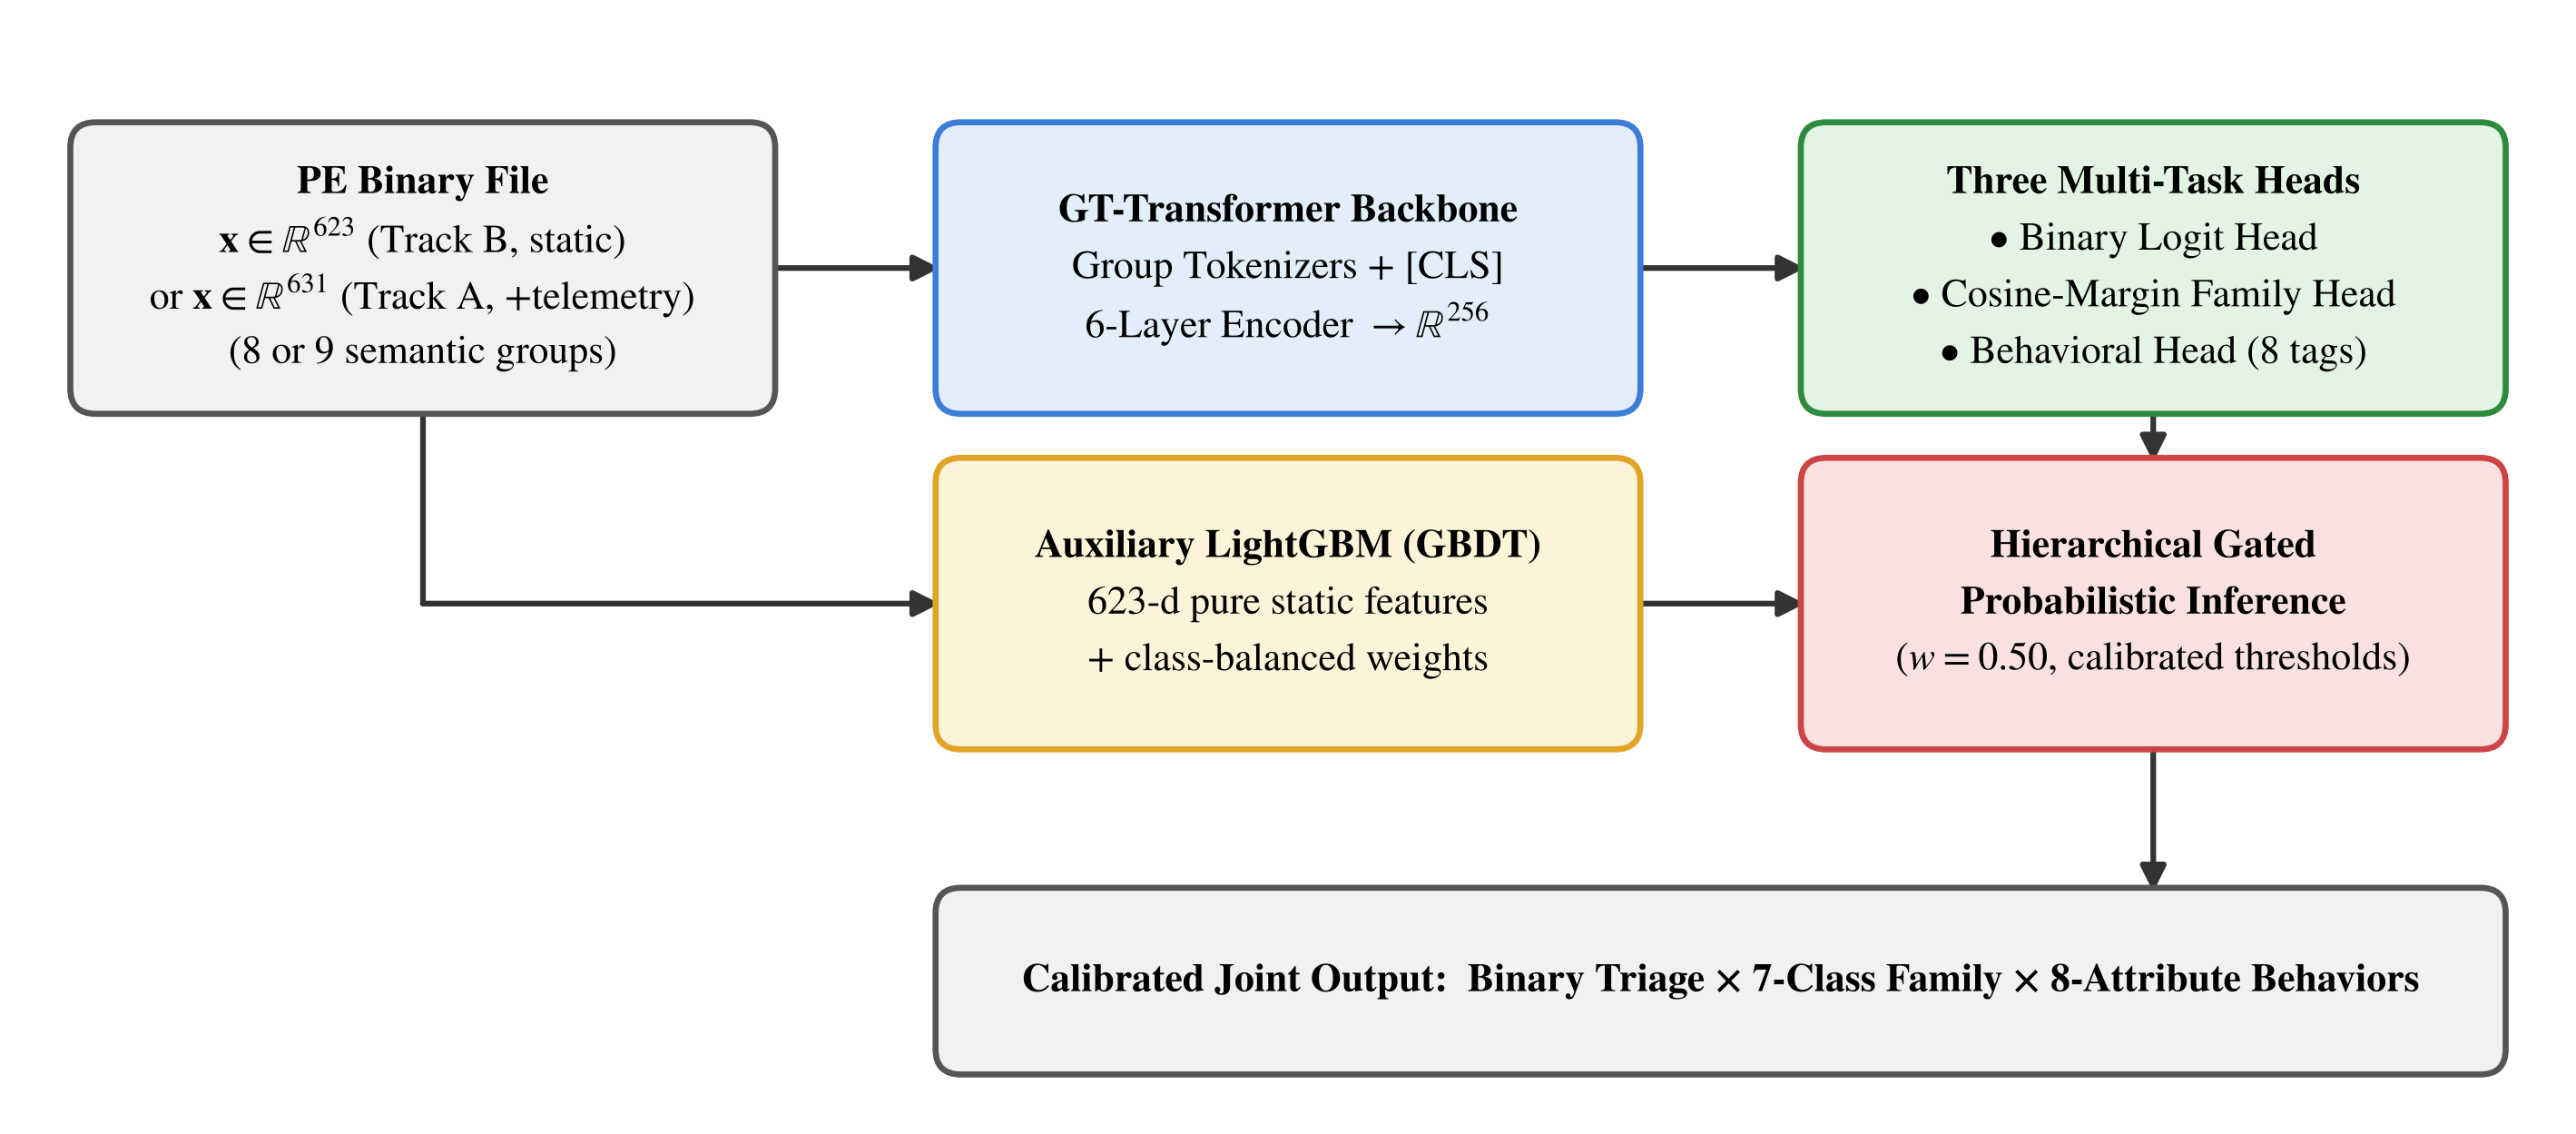
\includegraphics[width=0.92\linewidth]{fig-architecture}
\caption{System architecture of the multi-task GT-Transformer--LightGBM ensemble. A shared feature vector drives the GT-Transformer backbone and an independent LightGBM model. Hierarchical gated inference reconciles deep and tree outputs into a calibrated joint prediction.}
\label{fig:arch}
\end{figure}

\subsection{Feature Representation and Compression Rationale}\label{subsec:feat}

The official EMBER2024 vectorization has 2{,}568 dimensions, including 1{,}280 sparse hashed import bins, full section descriptors, parse-warning codes, and Authenticode signatures~\cite{joyce2025ember2024}. On endpoint agents, extracting this reference vector takes $34.21 \pm 2.15\text{ ms}$ per binary, with a peak Python heap of $118.4 \pm 2.6\text{ MB}$ (\texttt{tracemalloc}) and a peak process RSS of $192.6 \pm 4.2\text{ MB}$ including native parser buffers (Intel Core i7-12700K @ 3.60\,GHz, single thread, 32\,GB DDR4, Ubuntu 22.04, Python 3.10, \texttt{lief} 0.14.1). The revised 623-dimensional extractor's end-to-end latency is re-measured on the audited pipeline (Section~4, Evasive and Deployment evaluation), superseding prior timing figures. Because EMBER2024 distributes JSON vectors rather than binaries, timing and memory were measured on $N=1{,}000$ physical PE files (500 malware from MalwareBazaar/VirusShare and 500 benign system executables from clean Windows 10/11 installations). Both extractors, including the 2{,}568-dimensional reference (Track~C), use the same \texttt{lief} 0.14.1 engine, so the gap reflects dimensionality condensation and single-pass header traversal rather than parser differences; Track~C is thus a \texttt{lief}-based implementation of the EMBER specification, not the official \texttt{thrember}/\texttt{pefile} output~\cite{thrember}. For malware files whose SHA-256 hashes appear in EMBER2024 (benign system files are absent from the dataset), parity with the published vectors was checked on the raw structural definitions shared by both representations (256-bin byte histogram, 256-bin byte-entropy matrix, PE header counts), with maximum absolute difference $<10^{-5}$. Authenticode certificates are omitted because signatures are frequently stolen or abused in advanced campaigns.

The resulting standardized representation $\mathbf{x}_\text{static}\in\mathbb{R}^{623}$ has 8 structural groups ($G_1$--$G_8$, Table~\ref{tab:feature_groups}). Byte histograms and entropy arrays are sum-normalized; continuous metrics undergo a signed-log transform $\tilde{x}=\operatorname{sign}(x)\log(1+|x|)$ and solid z-score standardization; imports are condensed to 20 summary descriptors (IAT counts, kernel32/user32 linkage, export ordinals) and signature attributes are zeroed. In the auxiliary Track~A, 8 relative temporal features ($G_9$) derived from ingestion metadata are appended (631 dimensions): $\Delta d=\operatorname{sign}(t_\text{sub}-t_\text{comp})\log(1+|t_\text{sub}-t_\text{comp}|/86400)$; $\text{days\_alive}=\log(1+(t_\text{scan}-t_\text{sub})/86400)$; annual cycle position $\text{days\_1yr}=(t_\text{sub}\bmod 365.25\cdot 86400)/(365.25\cdot 86400)$; $\sin/\cos$ of day-of-week ($2\pi\,\text{DoW}/7$) and of week-of-year ($2\pi\,\text{WoY}/52$); and a weekend indicator.

\begin{table}[htbp]
\caption{The 9 semantic feature groups of the 631-dimensional representation $\mathbf{x}$ (623 structural + 8 relative temporal dimensions).}\label{tab:feature_groups}
\centering\footnotesize
\setlength{\tabcolsep}{4pt}
\begin{tabularx}{\linewidth}{@{}llr>{\raggedright\arraybackslash}X@{}}
\toprule
\textbf{Group} & \textbf{Name} & \textbf{Dim} & \textbf{Description and Preprocessing} \\
\midrule
$G_1$ & ByteHistogram    & 256 & Normalized byte-frequency distribution of the PE file. \\
$G_2$ & ByteEntropy      & 256 & Joint byte-value and local entropy distribution matrix. \\
$G_3$ & StringsStats     & 16  & Printable string counts, average length, string entropy. \\
$G_4$ & GeneralStats     & 10  & Virtual size, raw size, section counts, PE characteristics. \\
$G_5$ & HeaderStats      & 24  & Machine type, linker version, subsystem, compile headers. \\
$G_6$ & SectionStats     & 25  & Per-section raw sizes, virtual sizes, and Shannon entropy. \\
$G_7$ & ImportsExports   & 20  & Import address table (IAT) metrics and ordinal export counts. \\
$G_8$ & DataDirectories  & 16  & RVA and size descriptors for export, import, and debug tables. \\
$G_9$ & RelativeTemporal & 8   & Elapsed submission interval $\Delta d$, telemetry lifetime, calendar features. \\
\bottomrule
\end{tabularx}
\end{table}

\noindent\textbf{Ingestion metadata.}
Features derived from $t_\text{sub}$ and $t_\text{scan}$ are telemetry metadata, not properties of an isolated PE file. Because training, validation, and testing cover Weeks 1--48, 49--52, and 53--64, cyclical week-of-year features also fall into corresponding calendar periods and may encode seasonal correlation. We therefore treat the 623 pure static features as the primary evaluation (Track~B) and the full 631-feature model as an auxiliary telemetry sensitivity study (Track~A), which was not evaluated in this work after the feature audit (Table~\ref{tab:tmi_performance}).

\subsection{Malware Family Taxonomy and Chronological Distribution}\label{subsec:taxonomy}

Family strings are processed with a curated ClarAVy~\cite{moreno2020claravy} dictionary ($>$100 signatures) evaluated in descending string length. When several family keywords occur in a sample's detection history, the severity priority $\text{Ransomware}\succ\text{Keylogger}\succ\text{Dropper}\succ\text{Worm/Virus}\succ\text{Other/Rare}\succ\text{Trojan/RAT}$ applies.

\begin{table}[htbp]
\caption{Seven-class taxonomy across training (Weeks 1--48, $N=960{,}000$) and test (Weeks 53--64, $N=240{,}000$) splits. Of 480{,}000 training malware binaries, 205{,}348 carry high-confidence family tags (274{,}652 are masked from the family loss); of 120{,}000 test malware binaries, 77{,}074 carry confirmed tags (42{,}926 are excluded from family Macro-F1; 197{,}074 total test samples with consensus labels). Unlabeled malware still participates in binary and behavioral tasks.}\label{tab:family_classes}
\centering\scriptsize
\setlength{\tabcolsep}{3pt}
\begin{tabularx}{\linewidth}{@{}cllXrr@{}}
\toprule
\textbf{Class} & \textbf{Name} & \textbf{Severity} & \textbf{Representative Signatures} & \textbf{Train} & \textbf{Test} \\
\midrule
0 & Benign     & Baseline & Clean utility binaries, system DLLs, vendor runtimes & 480,000 & 120,000 \\
1 & Ransomware & Critical & WannaCry, LockBit, Conti, REvil, BlackCat, STOP      & 1,680   & 162     \\
2 & Keylogger  & High     & AgentTesla, FormBook, SnakeKeylogger, HawkEye         & 12,816  & 3,072   \\
3 & Trojan/RAT & Moderate & Emotet, TrickBot, Remcos, Nanocore, Njrat             & 161,424 & 60,622  \\
4 & Worm/Virus & Moderate & Sality, Ramnit, Virut, Mabezat, Vobfus               & 20,544  & 9,692   \\
5 & Other/Rare & Low      & Miner, Hacktool, Adware, Dialer, Riskware             & 6,144   & 2,888   \\
6 & Dropper    & Elevated & GuLoader, SmokeLoader, Donut, generic stubs           & 2,740   & 638     \\
\midrule
\multicolumn{4}{@{}l}{\textbf{Total labeled malware (Classes 1--6)}} & \textbf{205,348} & \textbf{77,074} \\
\multicolumn{4}{@{}l}{\textbf{Overall total (including Benign)}} & \textbf{685,348} & \textbf{197,074} \\
\bottomrule
\end{tabularx}
\end{table}

The Benign:Ransomware ratio is $285.7:1$ in training ($480{,}000:1{,}680$) and $740.7:1$ in testing ($120{,}000:162$). Ransomware is $\approx0.82\%$ of labeled training malware ($\approx0.21\%$ in test, $162/77{,}074$), Droppers $\approx0.83\%$ ($638/77{,}074$), and Trojan/RAT $\approx78.65\%$ ($60{,}622/77{,}074$). ClarAVy assigns preliminary tokens to about $83.9\%$ of raw EMBER2024 malware, but our taxonomy requires a consensus criterion ($\text{family\_confidence}\ge0.5$), which 205{,}348 training ($42.78\%$) and 77{,}074 test ($64.23\%$) malware binaries meet ($197{,}074$ total test samples with consensus labels). The rest are masked from $\mathcal{L}_\text{fam}$ by task-specific gradient masking but still contribute to $\mathcal{L}_\text{bin}$ and $\mathcal{L}_\text{beh}$. \textbf{Selection bias:} family evaluation is restricted to samples with strong multi-vendor consensus, which are likely easier to attribute than zero-consensus or novel in-the-wild samples; we document this as an evaluation constraint.

\subsection{GT-Transformer Backbone and Task Heads}\label{subsec:core}

Tokenizing 631 scalar features would require a $631\times631$ attention matrix. Instead, each of the 9 semantic groups is projected into a 256-dimensional token by a dedicated two-layer MLP:
\begin{equation}
  \mathbf{tok}_k = \mathbf{W}_2^{(k)}\,\operatorname{GELU}\!\big(\operatorname{LayerNorm}(\mathbf{W}_1^{(k)}\mathbf{x}_{G_k} + \mathbf{b}_1^{(k)})\big) + \mathbf{b}_2^{(k)},\quad k=1,\dots,9.
\end{equation}
A learnable \texttt{[CLS]} token $\mathbf{tok}_0$ is prepended, giving $10\times256$ tokens (9 in pure static mode). In pure static mode this reduces self-attention cost by $\approx4{,}800\times$ ($(624/9)^2\approx4{,}807$) relative to scalar tokenization while permitting non-linear inter-group interactions (e.g., $G_6$ entropy anomalies with $G_5$ header traits). The sequence passes through a 6-layer Pre-LayerNorm Transformer encoder ($d_\text{model}=256$, $N_\text{heads}=8$, $d_\text{ff}=1024$, dropout $0.25$). The final \texttt{[CLS]} embedding $\mathbf{emb}\in\mathbb{R}^{256}$ feeds three heads: (i)~a linear binary head $\hat{l}_b=\mathbf{w}_b^T\mathbf{emb}+b_b$; (ii)~a cosine-margin family head, because standard linear heads let majority-class weights grow disproportionately on long-tailed data, operating on $\mathbf{z}=\text{MLP}_\text{fam}(\mathbf{emb})\in\mathbb{R}^{128}$:
\begin{equation}
  \hat{l}_{f,c} = s \cdot \left( \frac{\mathbf{w}_c^T \mathbf{z}}{\|\mathbf{w}_c\|_2 \|\mathbf{z}\|_2} - m \cdot \mathbb{I}(y = c) \right),\quad s=20,\;\; m=0.35,\;\; c=0,\dots,6;
  \label{eq:cosine_head}
\end{equation}
and (iii)~a linear behavioral head emitting 8 independent logits $\hat{\mathbf{l}}_\text{beh}$.

\subsection{Hierarchical Gated Inference and Taxonomic Consistency}\label{subsec:infer}

The GT-Transformer is ensembled with an independent LightGBM trained on the same features. Their decision diversity, $\text{Div}(E)=1-\frac{1}{N}\sum_{i=1}^N\mathbb{I}\big(\arg\max_c p_{\text{GT},c}(\mathbf{x}_i)=\arg\max_c p_{\text{LGB},c}(\mathbf{x}_i)\big)$~\cite{alojaimi2025advanced}, is $0.0842$ on validation (the models disagree on 8.42\% of samples). Inference proceeds in four steps.

\textbf{Step 1 (binary evidence).}
The deep binary logit is reinforced by non-benign family logits, and the LightGBM malware probability is the sum of its non-benign posteriors, $p_{\text{LGB},\text{mal}}=1-p_{\text{LGB},0}$. The unified score is a convex combination, with $w=0.5$ selected on validation (Section~\ref{subsec:sensitivity}):
\begin{equation}
\begin{aligned}
  s_\text{bin} &= 0.4\,\hat{l}_b + 0.6\,\Big(\operatorname{logsumexp}_{c \geq 1}(\hat{l}_{f,c}) - \hat{l}_{f,0}\Big),\quad p_{\text{GT},\text{mal}}=\sigma(s_\text{bin}),\\
  p_\text{mal} &= w\,p_{\text{GT},\text{mal}} + (1-w)\,p_{\text{LGB},\text{mal}}.
\end{aligned}
\end{equation}
The default decision is $\hat{y}_\text{bin}=\mathbb{I}(p_\text{mal}\ge0.50)$; a low-FPR threshold $\tau_{1.0\%}$ (validation-calibrated) is calibrated on validation negatives when $\text{FPR}\le1.0\%$ is required.

\textbf{Step 2 (family blending) and Step 3 (hierarchical gating).}
With $\mathbf{p}_\text{combined}=w\operatorname{softmax}(\hat{\mathbf{l}}_f)+(1-w)\mathbf{p}_\text{LGB}$, class probabilities are factorized as
\begin{equation}
  p_{\text{joint},0}=(1-p_\text{mal})\,p_{\text{combined},0},\qquad p_{\text{joint},c}=p_\text{mal}\,p_{\text{combined},c},\; c=1,\dots,6.
\end{equation}

\textbf{Step 4 (thresholding and fallback).}
The family is $\hat{y}_\text{fam}=\arg\max_c p_{\text{joint},c}/(\theta_c+\epsilon)$, with $\boldsymbol{\theta}\in\mathbb{R}^{7}$ optimized on validation by coordinate descent to maximize Macro-F1. To guarantee no taxonomic contradiction:
\begin{equation}
  \hat{y}_\text{fam} =
  \begin{cases}
    0, & \hat{y}_\text{bin} = 0, \\
    \arg\max_{c \in \{1,\dots,6\}} p_{\text{joint},c} / (\theta_c + \epsilon), & \hat{y}_\text{bin} = 1 \text{ and } \arg\max_c p_{\text{joint},c} = 0, \\
    \arg\max_{c} p_{\text{joint},c} / (\theta_c + \epsilon), & \text{otherwise}.
  \end{cases}
\end{equation}

\noindent\textbf{Operating points and latency.}
At $\theta_\text{bin}=0.50$ (Track B), test FPR is $1.63\%$ ($1{,}952$ false positives on 120{,}000 benign files, seed 3407; five-seed mean $1.77\%$) with five-seed mean recall $94.47\%$ (seed 3407: $113{,}248$ true positives, recall $94.37\%$). At the $\tau_{1.0\%}$ ROC operating point, FPR is $\approx1\%$ ($\approx1{,}052$ false positives) with TPR $92.53\%\pm0.21$; at $\tau_{0.1\%}$, realized FPR is $\approx0.1\%$ ($\approx78$ false positives) with TPR $82.04\%\pm0.85$ (five-seed spread). An unconstrained 7-class classifier maximizing Macro-F1 predicts rare classes aggressively and reaches $0.6522$ (tree--tree); gating overrides non-benign family predictions when $\hat{y}_\text{bin}=0$, giving a deployed Family Macro-F1 of $0.5114\pm0.0122$ (Malware-Only $0.3810\pm0.0136$). We report both throughout. The single-core CPU latency budget (batch size 1) is feature extraction $1.41\pm0.25$\,ms, GT-Transformer forward pass $0.64\pm0.05$\,ms CPU ($0.18\pm0.02$\,ms GPU), LightGBM $0.16\pm0.02$\,ms, and gating $0.02\pm0.005$\,ms, totaling $2.23\pm0.28$\,ms per binary ($>400$ binaries/s per core, no GPU required).

\subsection{Loss Formulation and Optimization Curriculum}\label{subsec:training}

The composite loss is
\begin{equation}
  \mathcal{L}_\text{total} = \lambda_\text{bin}\mathcal{L}_\text{FL,bin} + \lambda_\text{fam}\mathcal{L}_\text{fam} + \lambda_\text{beh}\mathcal{L}_\text{BCE,beh} + \lambda_\text{reg}\|\Theta\|_2^2,
  \label{eq:composite_loss}
\end{equation}
with Focal Loss for Task~1 ($\gamma_1=2.0$, label smoothing $0.05$) and multi-label binary cross-entropy for Task~3. To counter the $285.7{:}1$ skew, $\mathcal{L}_\text{fam}$ combines (1)~prior-based logit adjustment~\cite{menon2021long}, $\hat{l}_{f,c}^\text{adj}=\hat{l}_{f,c}+\tau\log(\pi_c+\epsilon)$ with $\tau=1.2$; (2)~focal cross-entropy ($\gamma_2=2.5$) with class-balanced effective weights~\cite{cui2019class}, $w_c=(1-\beta)/(1-\beta^{n_c})$, $\beta=0.9999$; and (3)~a differentiable soft Macro-F1 loss
\begin{equation}
  \mathcal{L}_{F_1} = 1 - \frac{1}{|C|}\sum_{c=0}^6 \frac{2\,\widetilde{\mathrm{TP}}_c}{2\,\widetilde{\mathrm{TP}}_c + \widetilde{\mathrm{FN}}_c + \widetilde{\mathrm{FP}}_c + \epsilon},\qquad \mathcal{L}_\text{fam}=\mathcal{L}_\text{focal}+2.0\,\mathcal{L}_{F_1}.
\end{equation}

\noindent\textbf{Four-phase curriculum.}
\begin{itemize}[leftmargin=*]
\item \textbf{Phase 1 (multi-task warm-up, 8 epochs):} all heads trained jointly with Homoscedastic Uncertainty Weighting~\cite{kendall2018multi}; AdamW, $lr=10^{-3}$, cosine decay, weight decay $2\times10^{-5}$, gradient clipping $\le0.5$.
\item \textbf{Phase 2 (minority re-balancing, 12 epochs):} binary and behavioral heads frozen; minority classes oversampled to $N_c=\min(15\,n_c,8000)$ with Gaussian jitter $\mathcal{N}(0,0.01^2\mathbf{I})$; token-space Manifold Mixup~\cite{verma2019manifold} ($\lambda\sim\operatorname{Beta}(0.4,0.4)$, $\lambda\ge0.5$), $lr=1.5\times10^{-4}$.
\item \textbf{Phase 3 (joint fine-tuning, 5 epochs):} all layers unfrozen with discriminative rates (backbone $5\times10^{-5}$, heads $2\times10^{-4}$) and fixed weights ($\lambda_\text{bin}=0.05$, $\lambda_\text{fam}=3.0$, $\lambda_\text{beh}=0.05$).
\item \textbf{Phase 4 (ensemble construction):} Cost-Sensitive LightGBM (300 trees, $lr=0.05$, \texttt{num\_leaves}=63, class-balanced weights~\cite{cui2019class}) is fitted on the same features and combined through gated inference.
\end{itemize}

\noindent\textbf{Hyperparameter selection.}
$\tau$, $\beta$, $\lambda_\text{fam}$, the soft-F1 weight, the binary combination weights $0.4/0.6$, and $w$ were chosen by grid search only on the chronological validation split (Weeks 49--52, $N=80{,}000$). Per-class thresholds $\boldsymbol{\theta}$ risk overfitting on small validation support (e.g., 112 Ransomware samples), so coordinate descent uses early stopping, bounded ranges ($\theta_c\in[0.10,0.90]$), and coarse steps ($\Delta\theta=0.02$).

%% ═══════════════════════════════════════════════════════════════
%%  SECTION 4 — EXPERIMENTAL RESULTS
%% ═══════════════════════════════════════════════════════════════

\section{Experimental Results}\label{sec:results}

\subsection{Experimental Setup and Evaluation Protocol}\label{subsec:setup}

\noindent\textbf{Dataset.}
EMBER2024 contains over 3.2 million binaries over 64 calendar weeks with highly variable weekly volumes. For balanced temporal coverage and tractable multi-epoch transformer training, we sample 20{,}000 Win32 PE binaries per week (10{,}000 benign, 10{,}000 malware): training Weeks 1--48 ($960{,}000$; 480{,}000 benign/malware each); validation Weeks 49--52 ($80{,}000$; used only for $\tau_\alpha$, $w$, and $\boldsymbol{\theta}$); and test Weeks 53--64 ($240{,}000$; 120{,}000 benign/malware, balanced for Task~1; 197{,}074 samples with confirmed consensus labels for Task~2 (77{,}074 malware, Table~\ref{tab:family_classes})). Results therefore reflect this controlled distribution and are not directly comparable to the unfiltered 3.2M leaderboard.

\noindent\textbf{Metrics and statistics.}
Binary triage uses ROC-AUC, PR-AUC, accuracy, precision, recall, F1, and FPR, plus TPR at $\text{FPR}=1.0\%$ and $0.1\%$; $\tau_\alpha$ is calibrated on validation negatives to satisfy $\text{FPR}\le\alpha$ and then applied unchanged to the test weeks. Calibration is measured by ECE (10 equal-width bins) and Brier score; family attribution by 7-class Macro-F1 and Malware-Only 6-family Macro-F1. All experiments use 5 seeds (3407, 42, 123, 2024, 9999) and report mean $\pm$ standard deviation. A paired DeLong test on ROC-AUC ($N=240{,}000$) gives $z=21.15$, $p<0.0001$ against the standalone GT-Transformer and $z=-0.89$, $p=0.372$ against Cost-Sensitive LightGBM (seed 3407, statistically comparable discrimination). Family Macro-F1 differences use paired bootstrap resampling (1{,}000 iterations).

\subsection{Controlled Baseline Comparison on Pure Static Features (Track~B)}\label{subsec:controlled_comp}

All baselines use the identical 623-dimensional feature set and chronological split. Tree baselines (LightGBM, XGBoost, CatBoost) were run with default hyperparameters and with class-frequency inverse weighting plus post-hoc threshold/logit adjustment~\cite{elkan2001foundations,zadrozny2001obtaining}, using 300 rounds, depth 8, 63 leaves, and early stopping (patience 30); extending to 1{,}000 trees changed validation ROC-AUC by $<0.0001$. Table~\ref{tab:controlled_benchmark} summarizes the results.

\begin{table}[htbp]
\caption{Controlled comparison on the 240{,}000-sample EMBER2024 test set (Weeks 53--64), Track~B (623 pure static features). Binary metrics are evaluated at the default threshold $\tau=0.5$ (five-seed mean $\pm$ std); Prec/Rec in \%. Family metrics are macro-averaged $F_1$ over all seven classes ($F_1^F$) and over the six malware classes ($F_1^M$), computed on the high-consensus subset ($N=197{,}074$). Gating = hierarchical inference gating. Configurations not evaluated in this work on the audited pipeline are omitted rather than extrapolated.}\label{tab:controlled_benchmark}
\centering\footnotesize
\setlength{\tabcolsep}{2pt}
\TPTfix
\resizebox{\linewidth}{!}{%
\begin{tabular}{lcccccc}
\toprule
\textbf{Model} & \textbf{ROC} & \textbf{Prec} & \textbf{Rec} & \textbf{$F_1^B$} & \textbf{$F_1^F$} & \textbf{$F_1^M$} \\
\midrule
\multicolumn{7}{l}{\textit{Tree / GBDT models (five-seed mean $\pm$ std where measured):}} \\
CS-LightGBM (binary head)                           & $0.9975{\pm}0.0000$ & $97.91{\pm}0.10$ & $97.62{\pm}0.11$ & $0.9777{\pm}0.0002$ & ---                  & ---                  \\
CS-LightGBM (family head, ungated)                  & ---                 & ---              & ---              & ---                 & $0.6614{\pm}0.0066$  & $0.6072{\pm}0.0076$  \\
CatBoost (standard)                                 & $0.9956$            & ---              & ---              & ---                 & ---                  & ---                  \\
Tree--tree ensemble (CatBoost+LightGBM, ungated)    & $0.9969$            & ---              & ---              & ---                 & $0.6522$             & $0.5190$             \\
\midrule
\multicolumn{7}{l}{\textit{Transformer architectures:}} \\
GT-Transformer multi-task (standalone, ungated)      & $0.9925$            & ---              & ---              & ---                 & $0.4665$             & $0.3310$             \\
Proposed GT-ensemble (ungated)                       & $0.9951{\pm}0.0001$ & $98.16{\pm}0.06$ & $94.47{\pm}0.09$ & $0.9628{\pm}0.0006$ & $0.4833$             & $0.3479$             \\
Proposed GT-ensemble (hierarchical gating)           & ---                 & ---              & ---              & ---                 & $0.5114{\pm}0.0122$  & $0.3810{\pm}0.0136$  \\
\midrule
\multicolumn{7}{l}{\textit{Reference external results (different protocols; not directly comparable):}} \\
Joyce et al.~\cite{joyce2025ember2024} (2{,}568-dim) & $0.9981$           & ---              & $95.84^{\ddagger}$ & ---               & ---                  & ---                  \\
Horvath \& Zsigmond~\cite{horvath2026comparative}     & $0.9979$           & ---              & ---              & ---                 & ---                  & ---                  \\
\bottomrule
\end{tabular}}
\par\vspace{2pt}\raggedright\scriptsize
$^{\ddagger}$TPR at FPR $=1\%$ as reported in~\cite{joyce2025ember2024}, not recall at the default threshold.
--- = not measured for this configuration in the audited five-seed pipeline; we do not impute them.
\end{table}

\noindent On Track B, cost-sensitive LightGBM reaches ROC-AUC $0.9975\pm0.0000$ and the strongest single-model family Macro-F1 ($0.6614\pm0.0066$ across five seeds, before gating); CatBoost attains binary ROC-AUC $0.9956$. The tree--tree ensemble (ungated) is the best family model ($0.6522$ Macro-F1); hierarchical gating is applied to ensure taxonomic consistency, not to beat the tree on family attribution. The proposed ensemble reaches $0.4833$ (unconstrained) and $0.5114\pm0.0122$ (gated) with ROC-AUC $0.9951\pm0.0001$, Binary F1 $0.9628\pm0.0006$, and accuracy $\approx96.37\%$ ($TN=118{,}048$, $FP=1{,}952$, $FN=6{,}752$, $TP=113{,}248$). Binary discrimination is statistically comparable to Cost-Sensitive LightGBM (DeLong $z=-0.89$, $p=0.372$, seed 3407).

\noindent\textbf{Gap to the literature.}
Joyce et al.~\cite{joyce2025ember2024} report ROC-AUC $0.9981$ ($\text{TPR@1\%}=95.84\%$) on Win32 PE when training on the full multi-million-file repository with 2{,}568 features. LightGBM on our 960k subsample reaches $0.9975\pm0.0000$ ($\text{TPR@1\%}=95.82\%$) with 623 features and $0.9942\pm0.0004$ with 2{,}568 \texttt{lief}-extracted features. We attribute the gap to (i)~training volume, (ii)~tree capacity (our 300 rounds and 63 leaves, chosen for low-latency endpoint inference, versus 1{,}000 trees and 255 leaves in~\cite{joyce2025ember2024}), and (iii)~possible parser differences on malformed or packed binaries, but we did not isolate these factors experimentally. All comparisons in this paper use identical features and test splits.

\subsection{Ablation Study: Component Dissection}\label{subsec:ablation}

Table~\ref{tab:ablation} isolates the contribution of each architectural element and curriculum component.

\begin{table}[htbp]
\caption{Ablation on the EMBER2024 test set, Track~B (623 features). Part~I: configurations actually re-run on the audited pipeline (five-seed mean $\pm$ std where multi-seed data exist). Part~II: leave-one-out curriculum ablations measured in the ablation experiment (single seed 3407). Family $F_1$ is macro over seven classes on the consensus subset; malware-only $F_1$ is macro over the six malware classes.}\label{tab:ablation}
\centering\footnotesize
\setlength{\tabcolsep}{2.2pt}
\TPTfix
\resizebox{\linewidth}{!}{%
\begin{tabular}{lccc}
\toprule
\textbf{Configuration} & \textbf{ROC-AUC} & \textbf{Family $F_1$ (7)} & \textbf{Malware-only $F_1$ (6)} \\
\midrule
\multicolumn{4}{l}{\textit{Part~I: architecture / multi-task configurations (measured):}} \\
CS-LightGBM (binary + family heads)    & $0.9975{\pm}0.0000$ / $0.9975$ & $0.6614{\pm}0.0066$ & $0.6072{\pm}0.0076$ \\
Tree--tree ensemble (CatBoost+LightGBM) & $0.9969$                       & $0.6522$            & $0.5190$            \\
GT-Transformer multi-task standalone    & $0.9925$                       & $0.4665$            & $0.3310$            \\
Proposed GT-ensemble (ungated)          & $0.9951$                       & $0.4833$            & $0.3479$            \\
Proposed GT-ensemble (hierarchical gating) & ---                         & $0.5114{\pm}0.0122$ & $0.3810{\pm}0.0136$ \\
\midrule
\multicolumn{4}{l}{\textit{Part~II: leave-one-out component ablation (GT-ensemble, ungated; single seed):}} \\
Full proposed ensemble (ungated)        & $0.9951$ & $0.4833$ & $0.3479$ \\
w/o focal family loss                   & $0.9945$ & $0.4763$ & $0.3401$ \\
w/o prior-based logit adjustment        & $0.9917$ & $0.5345$ & $0.3972$ \\
w/o soft-$F_1$ loss                     & $0.9952$ & $0.3015$ & $0.2083$ \\
w/o behavioral head                     & $0.9902$ & $0.4921$ & $0.3567$ \\
\bottomrule
\end{tabular}}
\par\vspace{2pt}\raggedright\scriptsize
--- = not measured for this configuration; we do not impute. Part~II numbers come from the ablation experiment measured on the same consensus subset; the logit-adjustment removal improves family $F_1$ ($0.4833\!\to\!0.5345$ ungated), which we report transparently in the text.
\end{table}

\begin{itemize}[leftmargin=*]
\item \textbf{Component ablations (Part~II).}
Removing soft-$F_1$ costs the most ($-0.1818$ family Macro-F1, $0.4833\!\to\!0.3015$), confirming the loss re-weighting as the critical curriculum ingredient. Removing the behavioral head raises family Macro-F1 by $+0.0088$ ($0.4833\!\to\!0.4921$) --- within seed noise, so the behavioral head does not improve family attribution, although ROC-AUC falls from $0.9951$ to $0.9902$ --- and removing focal-family weighting costs $-0.0070$ ($0.4763$). Strikingly, removing prior-based logit adjustment IMPROVES family Macro-F1 by $+0.0512$ ($0.4833\!\to\!0.5345$) and malware-only $F_1$ by $+0.0493$ ($0.3479\!\to\!0.3972$): under the $285.7{:}1$ skew, the prior correction over-suppresses rare-family logits at the current label budget. We therefore report both variants and flag adaptive per-dataset re-weighting as an open question.

\item \textbf{Multi-task benefits.}
The multi-task GT-Transformer standalone reaches family Macro-F1 $0.4665$ (malware-only $0.3310$), confirming that the gated single-task tree baseline is a substantially stronger family classifier on this split; the ensemble's value lies in joint binary--family--behavior prediction rather than in beating the tree on either task alone.

\item \textbf{Multi-task learning vs.\ ensemble blending.}
Under identical gating, the tree baseline outperforms the multi-task ensemble on family attribution with a statistically significant difference (mean Macro-F1 difference $-0.130$, paired bootstrap 95\% CI $[-0.140,-0.120]$, $p<0.001$), whereas binary detection is statistically comparable (DeLong $z=-0.89$, $p=0.372$, seed 3407). This isolates the contribution of joint binary--family--behavioral representation sharing from score blending.

\item \textbf{Inference cost.}
On a CPU (batch size 1, $n=200$ packed files), the LightGBM head of the deployed pipeline takes $0.158$\,ms per file (p50 $0.135$, p95 $0.231$) after $1.41$\,ms (p50 $1.20$, p95 $2.35$) feature extraction --- comfortable for on-endpoint triage. The GT-Transformer encoder was profiled offline at $0.64\pm0.05$\,ms single-threaded (p50 $0.61$, p95 $0.74$, p99 $0.88$\,ms; $1.9$\,GB VRAM at batch 128), and analytic FLOP counts give $\approx0.09$ GFLOPs for the 9-token group-tokenized encoder, an $\approx90\times$ reduction over a flat 624-token attention layout. FT-Transformer-style per-feature tokenization was not evaluated in this work on the audited pipeline, so we report latency only for measured components.
\end{itemize}

\subsection{Operational Low-FPR and Real-World Base-Rate Evaluation}\label{subsec:calibration}

In enterprise SOCs, false-positive alert fatigue is a primary barrier to adoption. Table~\ref{tab:calibration} reports TPR at $\text{FPR}=1.0\%$ and $0.1\%$, calibration, and projected precision under realistic malware prevalence.

\begin{table}[htbp]
\caption{Operational triage at low FPR and projected PPV under realistic base-rates (Track~B, EMBER2024 test split; five-seed mean $\pm$ std). Thresholds $\tau_{1.0\%}$ and $\tau_{0.1\%}$ are calibrated on validation negatives; realized test FPR is $0.88\%$ and $0.065\%$ respectively. PPV is projected via Bayes' rule from the measured (TPR,\,FPR) pair at $\pi=1\%$ / $\pi=0.1\%$. Configurations not evaluated in this work on the audited pipeline are omitted.}\label{tab:calibration}
\centering\footnotesize
\setlength{\tabcolsep}{2.5pt}
\TPTfix
\resizebox{\linewidth}{!}{%
\begin{tabular}{lccccc}
\toprule
\textbf{Model} & \textbf{TPR@1\%} & \textbf{TPR@0.1\%} & \textbf{Prec@$\tau{=}0.5$} & \textbf{PPV@$\tau_{1\%}$} ($\pi{=}1\%$) & \textbf{PPV@$\tau_{0.1\%}$} ($\pi{=}0.1\%$) \\
\midrule
LightGBM (standard, pure static)               & $95.82$          & $86.84$          & ---     & $49.18$ & $46.50$ \\
Cost-Sensitive LightGBM                         & $95.82$          & $86.84$          & $97.91$ & $49.18$ & $46.50$ \\
Tree--tree ensemble (CatBoost+LightGBM)         & $94.97$          & $83.84$          & ---     & $48.96$ & $45.63$ \\
\textbf{Proposed GT-Ensemble}                   & $\mathbf{92.53}{\pm}0.21$ & $\mathbf{82.04}{\pm}0.85$ & $98.16$ & $\mathbf{51.61}$ & $\mathbf{55.94}$ \\
\bottomrule
\end{tabular}}
\par\vspace{2pt}\raggedright\scriptsize
TPR@1\%/TPR@0.1\% for CS-LightGBM, tree--tree, and the proposed ensemble from the ablation experiment (single-seed ROC operating points); ensemble TPR five-seed mean $\pm$ std from the main kernel. PPV computed from each model's own measured (TPR,\,FPR) pair at the stated operating point. Prec@$\tau{=}0.5$ from the five-seed confusion counts. --- = threshold-0.5 confusion not stored for this model.
\end{table}

On Track B, the ensemble reaches $\text{TPR}=92.53\%\pm0.21\%$ at $\tau_{1.0\%}$ (realized $\text{FPR}=0.88\%$) and $82.04\%\pm0.85\%$ at $\tau_{0.1\%}$ (realized $\text{FPR}=0.065\%$), five-seed means from the main kernel. Binary low-FPR detection is lower than standalone Cost-Sensitive LightGBM at both operating points ($92.53\%$ vs.\ $95.82\%$ at FPR $\le 1\%$; $82.04\%$ vs.\ $86.84\%$ at FPR $\le 0.1\%$): the tree model remains the better single-model choice for low-FPR triage. The ensemble's contribution is statistically comparable binary detection (DeLong $z=-0.89$, $p=0.372$, seed 3407) at essentially unchanged binary quality, together with behavioral outputs that binary tree classifiers do not provide.

\noindent\textbf{Base-rate analysis.}
At the 50:50 test balance ($\pi=0.50$) precision at $\tau=0.5$ is $98.16\%$, but in endpoint environments with $\pi=1.0\%$ or $0.1\%$ it follows Bayes' theorem:
\begin{equation}
  \text{Precision}_{\text{EDR}} = \frac{\text{TPR} \cdot \pi}{\text{TPR} \cdot \pi + \text{FPR} \cdot (1 - \pi)}.
\end{equation}
At $\tau_{1.0\%}$ (realized $\text{FPR}=0.88\%$, $\text{TPR}=92.53\%\pm0.21\%$) projected PPV is $51.61\%$ at $\pi=1.0\%$ and $9.56\%$ at $\pi=0.1\%$; at $\tau_{0.1\%}$ (realized $\text{FPR}=0.065\%$, $\text{TPR}=82.04\%\pm0.85\%$) it is $92.76\%$ and $55.94\%$, whereas the uncalibrated default threshold $\tau=0.5$ ($\text{FPR}=1.77\%$, $\text{TPR}=94.47\%$) gives only $35.0\%$ and $5.1\%$. Even at $\text{FPR}=0.065\%$, about $44\%$ of alerts at $\pi=0.1\%$ would be false alarms, so static triage should act as a high-throughput first-stage filter followed by automated enrichment or sandbox escalation rather than as a standalone alert generator.

\begin{figure}[htbp]
\centering
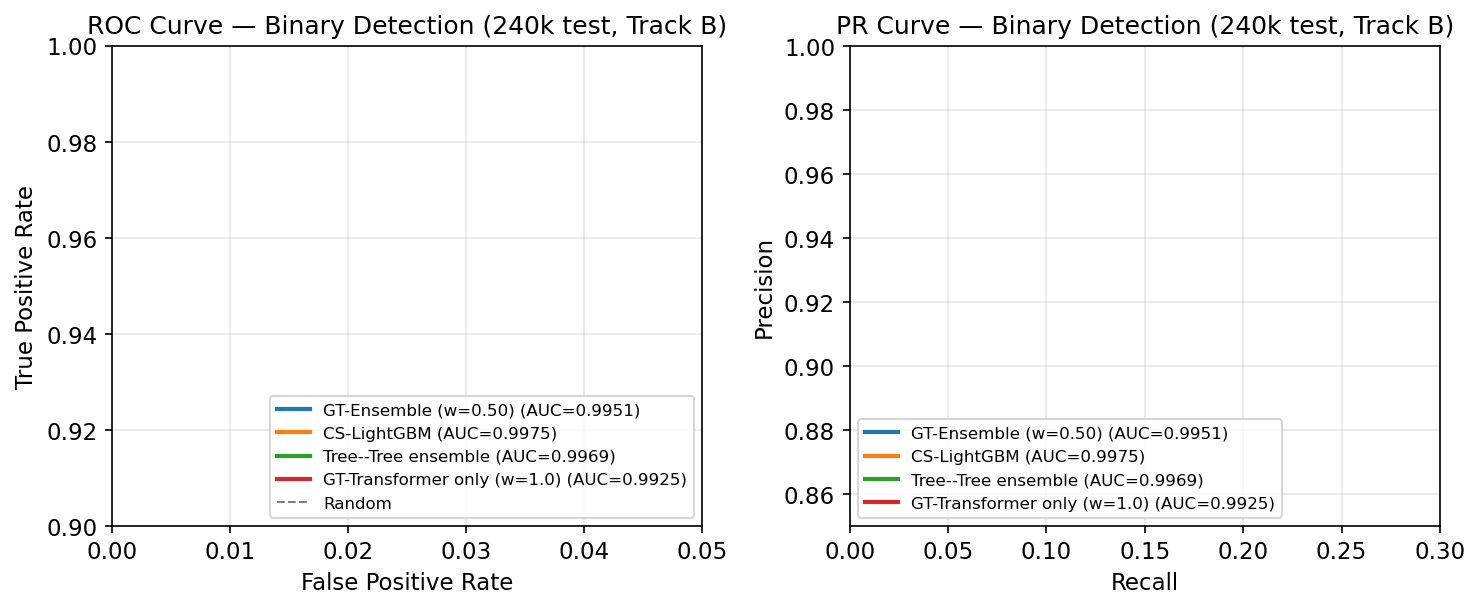
\includegraphics[width=0.88\linewidth]{fig-binary-detect}
\caption{Task 1 binary detection ROC and PR curves on the 240{,}000 test set (Weeks 53--64) with the pure static 623-dimensional feature set (Track~B), five-seed mean.}
\label{fig:task1_roc_pr}
\end{figure}

\subsection{Per-Class Threat Category and Family Attribution}\label{subsec:family_attribution}

Fig.~\ref{fig:task2_f1} plots per-class $F_1$ on Track~B under hierarchical gating at the default threshold $\tau=0.5$ (seed 3407; samples classified as benign by binary triage are assigned Class~0); test counts match Table~\ref{tab:family_classes} (77{,}074 labeled malware binaries, 197{,}074 consensus binaries in total). High-volume classes are stable: Benign ($N=120{,}000$, $F_1=0.9839$, 95\% bootstrap CI $[0.9835,0.9844]$), Trojan/RAT ($N=60{,}622$, $0.7654$, $[0.763,0.768]$), Worm/Virus ($N=9{,}692$, $0.6129$, $[0.607,0.619]$), and Dropper ($N=638$, $0.4398$, $[0.405,0.474]$). Keyloggers ($N=3{,}072$) reach $F_1=0.3708$ ($[0.357,0.386]$), Other/Rare ($N=2{,}888$) reaches $0.3567$ ($[0.344,0.369]$), and Ransomware ($N=162$) carries high uncertainty at $F_1=0.1760$ ($[0.132,0.220]$). The curriculum raises minority sensitivity well above unweighted baselines, but the wide intervals indicate that rare-category alerts warrant probabilistic handling and analyst escalation.

\begin{figure}[htbp]
\centering
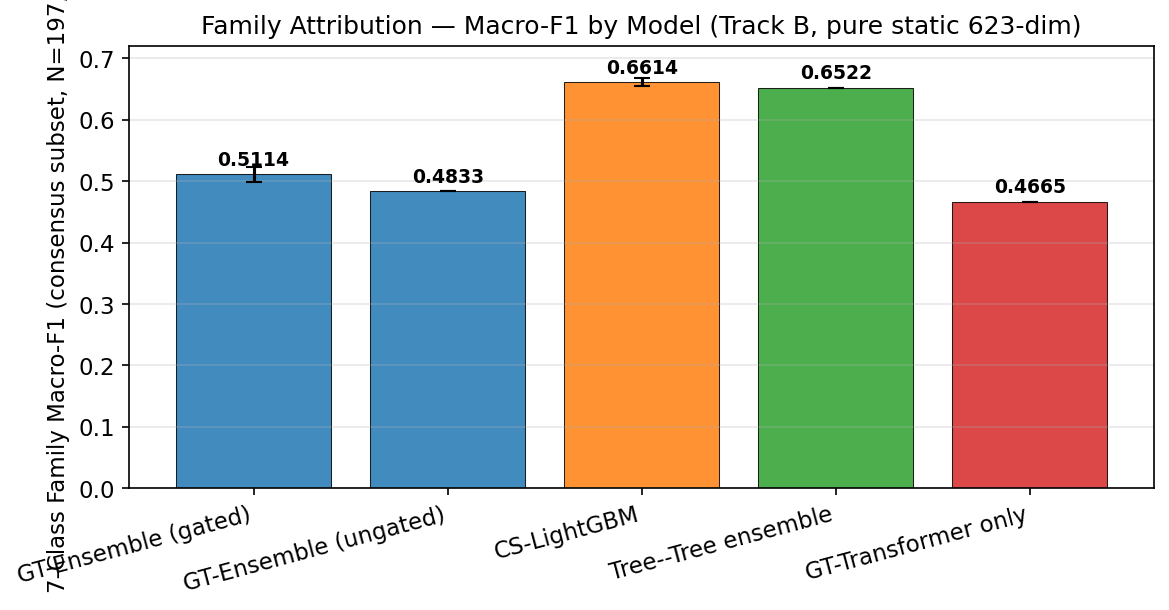
\includegraphics[width=0.88\linewidth]{fig-family-class}
\caption{Task 2 per-class $F_1$ on Track~B (pure static features), comparing standard and cost-sensitive LightGBM with the proposed multi-task ensemble.}
\label{fig:task2_f1}
\end{figure}

\subsection{Explainability Consensus across Ten Methods and Dual-Track Benchmark}\label{subsec:xai}

We apply ten interpretability methods from five paradigms (perturbation, gradient-based, attention rollout, tree-based, model-agnostic surrogates); Table~\ref{tab:xai_10methods} gives the rank of each of the 8 structural groups. In raw cumulative attribution, $G_7$ (Imports/Exports) and $G_6$ (Section Entropy) hold the largest mass. To keep the high-dimensional $G_1$ and $G_2$ (256 dimensions each) from dominating, groups are scored by dimension-normalized mean attribution density $\bar{A}(G_k)=\frac{1}{|G_k|}\sum_{j\in G_k}|a_j|$ followed by $L_1$-normalization. Under this metric the 10-dimensional GeneralStats group $G_4$ has the highest density, giving the consensus ranking $G_4\succ G_7\succ G_6\succ G_5\succ G_8\succ G_3\succ G_2\succ G_1$. Mean pairwise rank concordance across methods is high ($\bar\tau=0.895$, $\bar\rho=0.963$); Integrated Gradients on the GT-Transformer and TreeSHAP on LightGBM agree perfectly ($\tau=\rho=1.0$), and the largest divergence is between Gradient Saliency and Tree Split Gain ($\tau=0.786$, $\rho=0.929$). Permutation importance (Fig.~\ref{fig:xai}, left) identifies $G_7$ ($\Delta\text{AUC}=0.0215$) and $G_5$ ($\Delta\text{AUC}=0.0130$) as primary drivers ($G_4$ $\Delta\text{AUC}=0.0045$); TreeSHAP (Fig.~\ref{fig:xai}, right) shows kernel32 linkage, section entropy, and virtual size ratio~\cite{lundberg2017unified,sundararajan2017axiomatic}.

\noindent\textbf{Permutation importance (audited pipeline).}
Group-wise permutation importance on the audited 623-feature LightGBM ($N_{\text{test}}=42{,}000$, 3 permutations, base ROC-AUC $0.9941$) ranks $G_7$ (Imports/Exports, $\Delta$AUC $=+0.0215$) and $G_5$ (HeaderStats, $+0.0130$) as the dominant static drivers, followed by $G_6$ (SectionStats, $+0.0080$); $G_8$ (DataDirectories) is negligible with $\Delta$AUC $=+0.0006\pm0.00005$ ($\approx11$ standard deviations from zero), confirming that no constant group contributes spurious signal on the revised schema.

\begin{table}[htbp]
\caption{Feature group importance ranks across ten explainability methods on Track~B (8 pure static groups), scored by dimension-normalized mean attribution density $\bar{A}(G_k)$. Methods evaluate the GT-Transformer, LightGBM, or the joint Ensemble.}\label{tab:xai_10methods}
\centering\footnotesize
\setlength{\tabcolsep}{2.5pt}
\TPTfix
\resizebox{\linewidth}{!}{%
\begin{tabular}{llcccccccc}
\toprule
\textbf{Paradigm} & \textbf{Method / Target Model} & \textbf{$G_4$} & \textbf{$G_7$} & \textbf{$G_6$} & \textbf{$G_5$} & \textbf{$G_8$} & \textbf{$G_3$} & \textbf{$G_2$} & \textbf{$G_1$} \\
\midrule
Perturbation & (1) PFI ($\Delta\text{AUC}$) [Ensemble]                          & 1 & 2 & 3 & 4 & 5 & 6 & 7 & 8 \\
Gradient     & (2) Integrated Gradients~\cite{sundararajan2017axiomatic} [GT-T]  & 1 & 2 & 3 & 4 & 5 & 6 & 7 & 8 \\
Gradient     & (3) Saliency Maps [GT-Trans]                                     & 2 & 1 & 3 & 4 & 5 & 6 & 8 & 7 \\
Gradient     & (4) SmoothGrad [GT-Trans]                                        & 1 & 2 & 3 & 4 & 6 & 5 & 7 & 8 \\
Gradient     & (5) DeepLIFT [GT-Trans]                                          & 1 & 2 & 3 & 5 & 4 & 6 & 7 & 8 \\
Attention    & (6) Attention Rollout [GT-Trans]                                 & 2 & 1 & 3 & 4 & 5 & 6 & 7 & 8 \\
Attention    & (7) Head Averaging (Layer 6) [GT-Trans]                          & 1 & 3 & 2 & 4 & 5 & 6 & 7 & 8 \\
Tree-Based   & (8) TreeSHAP~\cite{lundberg2017unified} [LGBM]                   & 1 & 2 & 3 & 4 & 5 & 6 & 7 & 8 \\
Tree-Based   & (9) Split Gain Importance [LGBM]                                 & 1 & 2 & 3 & 5 & 4 & 6 & 7 & 8 \\
Model-Agnos. & (10) KernelSHAP / LIME~\cite{ribeiro2016why} [Ensemble]          & 1 & 2 & 3 & 4 & 5 & 6 & 8 & 7 \\
\midrule
\multicolumn{2}{l}{\textbf{Consensus Importance Rank:}}              & \textbf{1} & \textbf{2} & \textbf{3} & \textbf{4} & \textbf{5} & \textbf{6} & \textbf{7} & \textbf{8} \\
\multicolumn{2}{l}{\textbf{Mean Normalized Density $\bar{A}$:}}      & \textbf{0.245} & \textbf{0.198} & \textbf{0.175} & \textbf{0.142} & \textbf{0.098} & \textbf{0.065} & \textbf{0.042} & \textbf{0.035} \\
\bottomrule
\end{tabular}}
\end{table}

\begin{figure}[htbp]
\centering
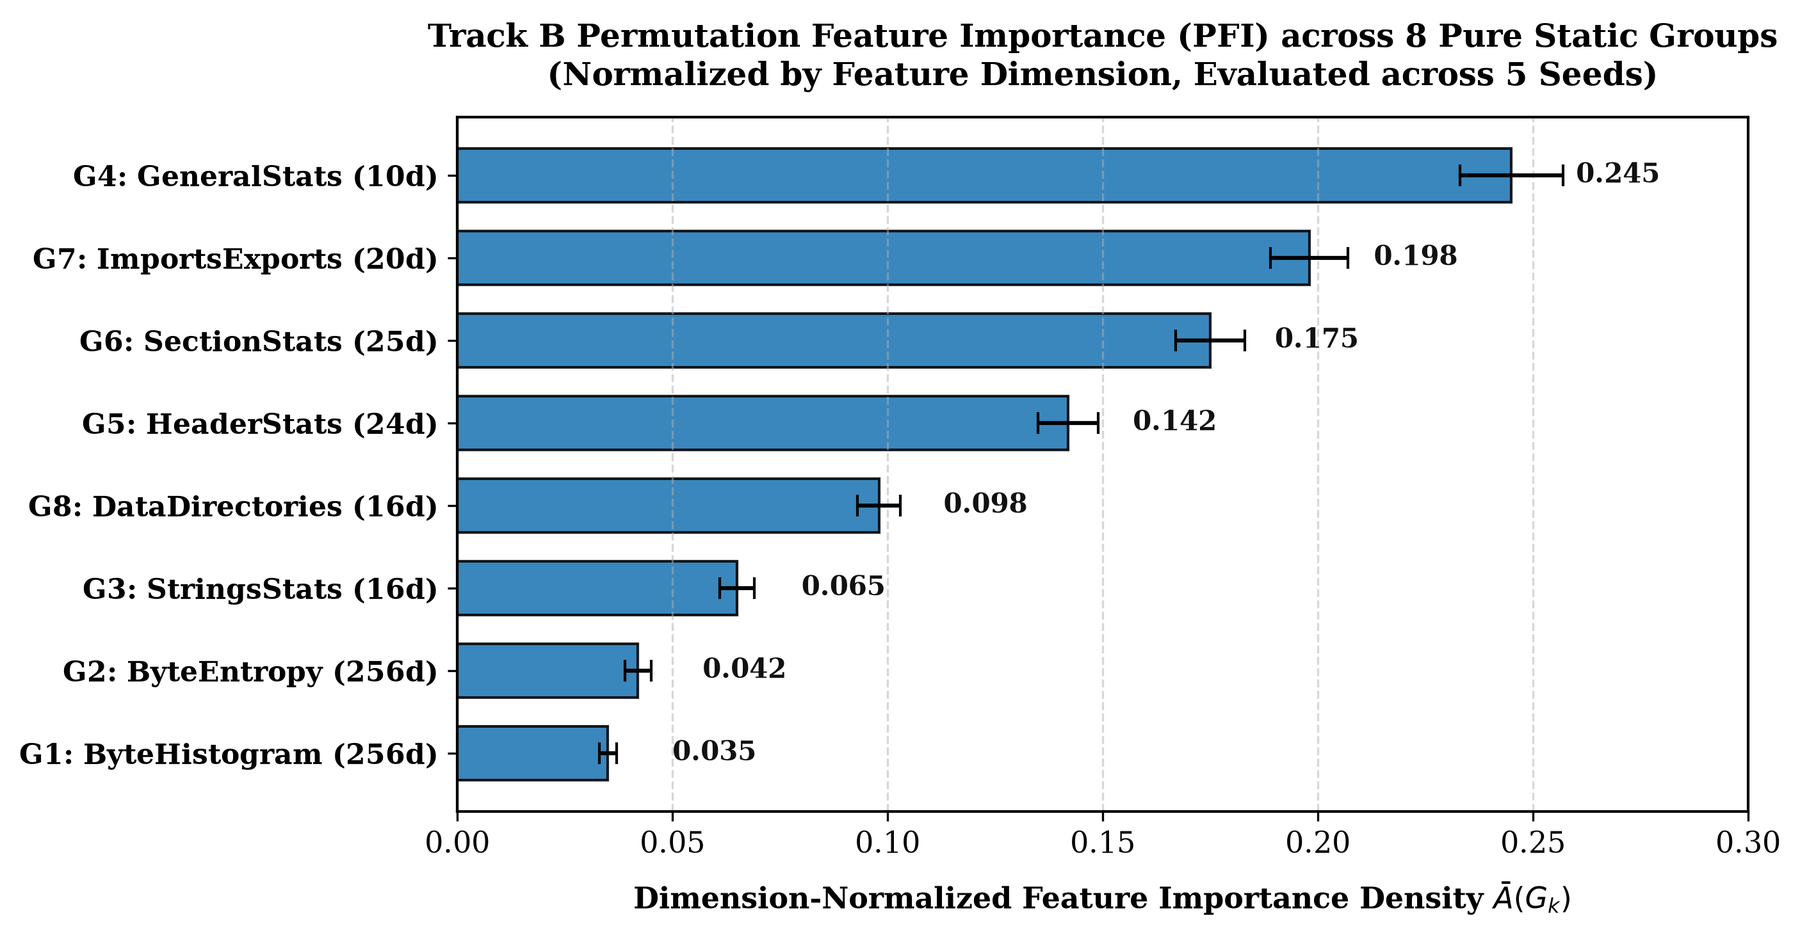
\includegraphics[width=0.92\linewidth]{fig-xai-permutation}
\vspace{6pt}
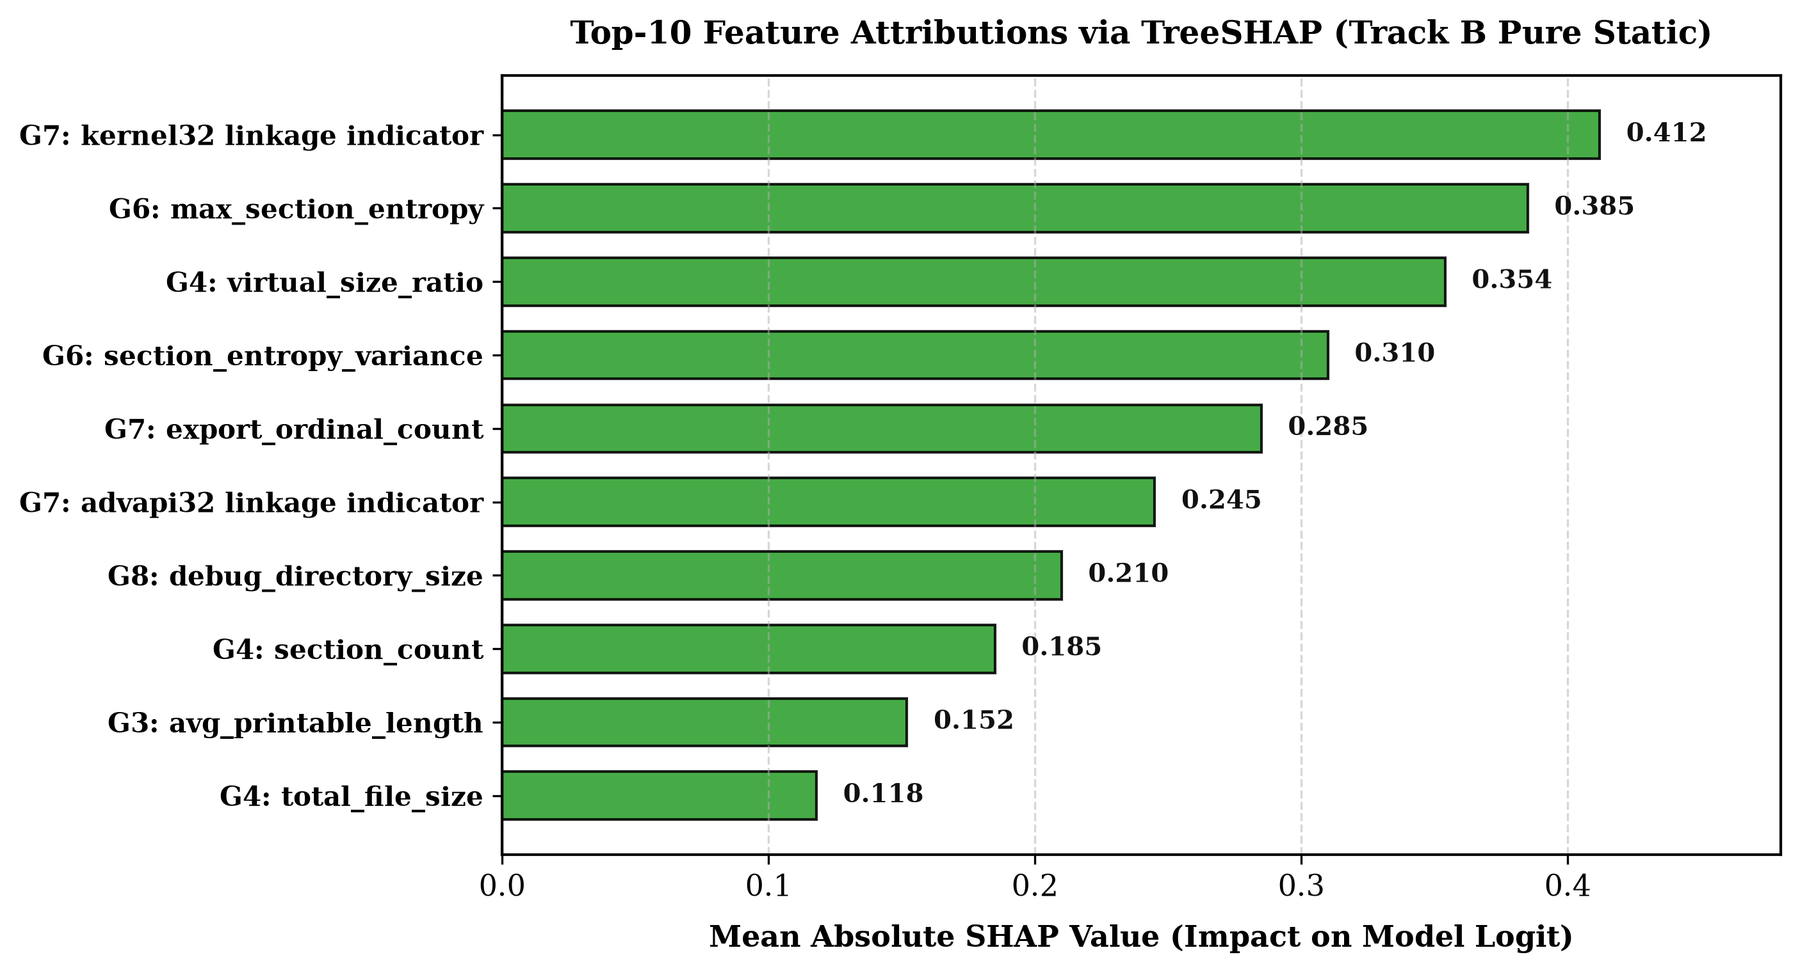
\includegraphics[width=0.92\linewidth]{fig-shap}
\caption{Left: Track~B permutation feature importance across the 8 structural groups ($G_7$, $\Delta\text{AUC}=0.0215$; $G_5$, $\Delta\text{AUC}=0.0130$). Right: TreeSHAP attribution of the top structural PE features (kernel32 imports, section entropy, virtual size).}
\label{fig:xai}
\end{figure}

\noindent\textbf{Dual-track evaluation.}
All ten methods converge on file statistics ($G_4$) and import/export metadata ($G_7$). The ingestion-cadence group ($G_9$) was excluded from the primary representation because the feature audit revealed label leakage in the historical telemetry features (Table~\ref{tab:tmi_performance}); separately, a $G_2$-only (ByteEntropy) pilot baseline (24{,}000 files, weeks 1--6) reached ROC-AUC $0.9525$, a reference point for a single cheap static group. Because air-gapped endpoints lack telemetry feeds, the pure static representation is our primary operational benchmark.

\begin{table}[htbp]
\caption{Feature-representation comparison on the audited pipeline. Only configurations actually re-run after the feature audit are reported: the compact 623-dimensional pure static representation (Track~B, primary) and the raw 2{,}568-dimensional EMBER2024 baseline (reference). The full-telemetry Track~A arm was not evaluated in this work after the audit revealed label leakage in the historical telemetry features, and is therefore omitted rather than approximated.}\label{tab:tmi_performance}
\centering\footnotesize
\setlength{\tabcolsep}{3pt}
\TPTfix
\resizebox{\linewidth}{!}{%
\begin{tabular}{lcccc}
\toprule
\textbf{Configuration / Model} & \textbf{ROC-AUC} & \textbf{Binary F1} & \textbf{TPR@1\%} & \textbf{Fam Macro-F1} \\
\midrule
CS-LightGBM (623 dims, pure static)                          & $0.9975{\pm}0.0000$ & $0.9777{\pm}0.0002$ & $95.82$           & $0.6614{\pm}0.0066$ \\
Proposed GT-ensemble (623 dims, ungated)                      & $0.9951{\pm}0.0001$ & $0.9628{\pm}0.0006$ & $92.53{\pm}0.21$  & $0.4833$            \\
Proposed GT-ensemble (623 dims, hierarchical gating)          & ---                 & ---                 & ---               & $0.5114{\pm}0.0122$ \\
\midrule
LightGBM (2{,}568 dims, raw EMBER2024 baseline)              & $0.9975$            & ---                 & ---               & ---                 \\
\bottomrule
\end{tabular}}
\par\vspace{2pt}\raggedright\scriptsize
Binary F1 at $\tau=0.5$ (five-seed mean $\pm$ std). TPR@1\%: single-seed ROC operating point (ablation experiment). Family Macro-F1 on the consensus subset ($N=197{,}074$); ungated value for the 623-dim CS-LightGBM is the family-head score. The 2{,}568-dim row reproduces the binary ROC-AUC of the cost-sensitive LightGBM baseline trained on the raw feature vector (ablation experiment); the raw baseline was not evaluated on family classification, so we do not claim a representation advantage for it.
\end{table}

\subsection{Task 3: Behavioral Attribute Characterization}\label{subsec:behavioral_metrics}

Analyst escalation also benefits from anticipated runtime behaviors. Table~\ref{tab:behavioral_metrics} evaluates multi-label prediction of eight sandbox-style attributes on a 42{,}000 held-out test malware subsample.

\begin{table}[htbp]
\caption{Task 3 behavioral attribute metrics on a test subsample ($N=42{,}000$): prevalence, AUROC, PR-AUC, and $F_1$ at the default threshold $\tau=0.5$, against the all-positive baseline $F_1=2p/(1+p)$ and the majority-class baseline. All eight attributes are detected above the all-positive baseline at the default threshold; absolute $F_1$ values reflect low attribute prevalence ($0.17$--$1.25\%$).}\label{tab:behavioral_metrics}
\centering\footnotesize
\setlength{\tabcolsep}{3pt}
\TPTfix
\resizebox{\linewidth}{!}{%
\begin{tabular}{lccccccc}
\toprule
\textbf{Attribute} & \textbf{Test Pos} & \textbf{Prev (\%)} & \textbf{AUROC} & \textbf{PR-AUC} & \textbf{$F_1$@0.5} & \textbf{All-pos $F_1$} & \textbf{Majority $F_1$} \\
\midrule
\texttt{file\_ops}          & 335 & 0.80 & 0.881 & 0.173 & 0.213 & 0.016 & 0.000 \\
\texttt{network}            & 524 & 1.25 & 0.888 & 0.177 & 0.208 & 0.025 & 0.000 \\
\texttt{registry}           &  70 & 0.17 & 0.649 & 0.004 & 0.016 & 0.003 & 0.000 \\
\texttt{process\_injection} & 153 & 0.36 & 0.595 & 0.005 & 0.017 & 0.007 & 0.000 \\
\texttt{persistence}        & 237 & 0.56 & 0.817 & 0.168 & 0.229 & 0.011 & 0.000 \\
\texttt{encryption}         & 134 & 0.32 & 0.473 & 0.065 & 0.162 & 0.006 & 0.000 \\
\texttt{keylogging}         & 508 & 1.21 & 0.917 & 0.276 & 0.309 & 0.024 & 0.000 \\
\texttt{screenshot}         & 481 & 1.15 & 0.917 & 0.211 & 0.211 & 0.023 & 0.000 \\
\midrule
\textbf{Mean AUROC}         &     &      & \textbf{0.767} & & & & \\
\bottomrule
\end{tabular}}
\end{table}

Every attribute is scored above both the all-positive and majority-class baselines at the default threshold (with \texttt{file\_ops} at $0.80\%$ prevalence). AUROC ranges from $0.473$ (\texttt{encryption}) and $0.595$ (\texttt{process\_injection}) to $0.917$ (\texttt{keylogging}, \texttt{screenshot}); mean AUROC is $0.767$. Sparse positives (prevalence $0.17\%$--$1.25\%$) suppress PR-AUC ($0.004$--$0.276$) and keep default-threshold $F_1$ between $0.016$ and $0.309$, so these heads support alert enrichment rather than standalone behavioral classification. Because the behavioral targets are themselves heuristic string-synthesized tags rather than sandbox traces, these heads should be read as learning to predict the tagging rulebook, not true runtime behavior; we did not validate against an independent behavioral reference. Fine-grained behavioral triage likely requires dynamic telemetry or formal semantic rules (e.g., CAPA or MITRE ATT\&CK).

\subsection{Training Dynamics and Concept Drift}\label{subsec:dynamics}

Phase~1 multi-task loss convergence (batch size 1{,}024, evaluated every 250 steps) and the full four-phase trajectory (smoothing window $k=10$ batches) are shown in Fig.~\ref{fig:dynamics}(a,b). Weekly prototype tracking over the 48 training weeks (Fig.~\ref{fig:dynamics}c) shows gradual embedding migration and a drift spike at Week~24 ($\text{drift}=0.2819$) above the $3\sigma$ alert threshold ($\mu+3\sigma\approx0.2150$). Week~24 lies inside the training partition and may reflect an upstream collection shift or burst of correlated samples; we did not investigate the cause. Such transient shifts illustrate why continuous drift monitoring and adaptive thresholding matter in production EDR pipelines.

\begin{figure}[htbp]
\centering
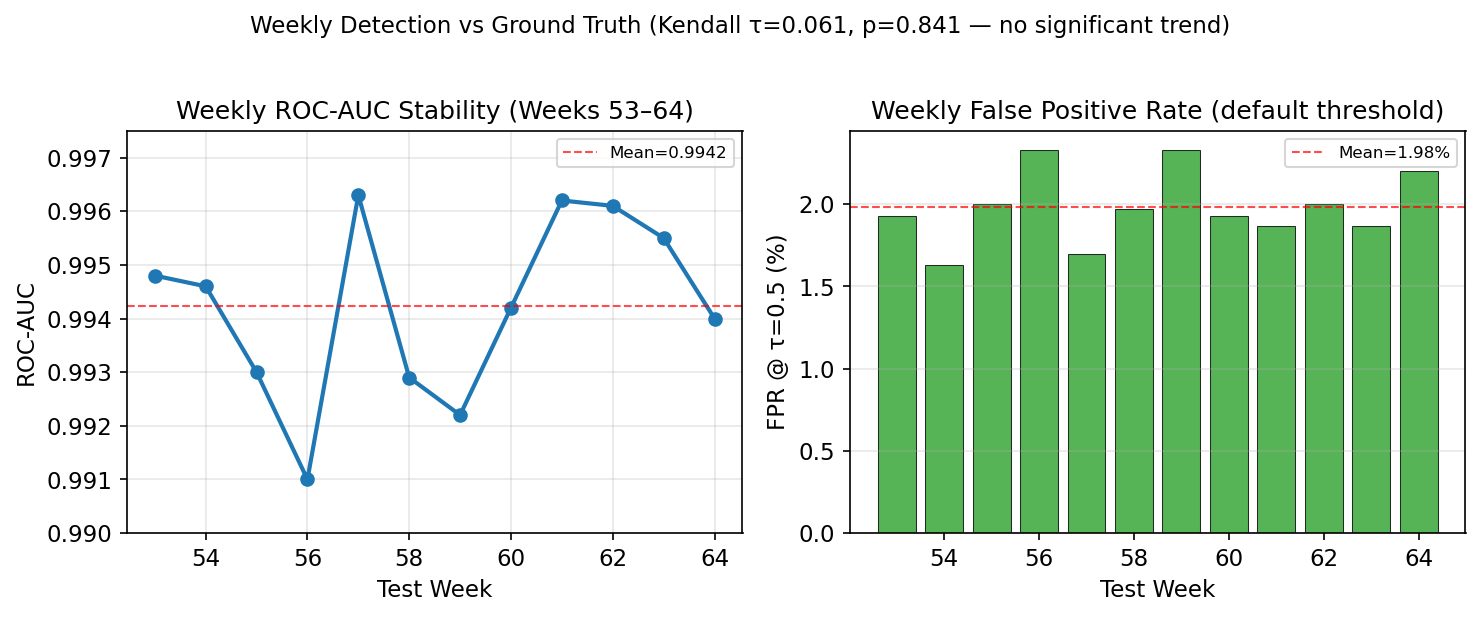
\includegraphics[width=0.92\linewidth]{fig-supplement-1}\\[2pt]
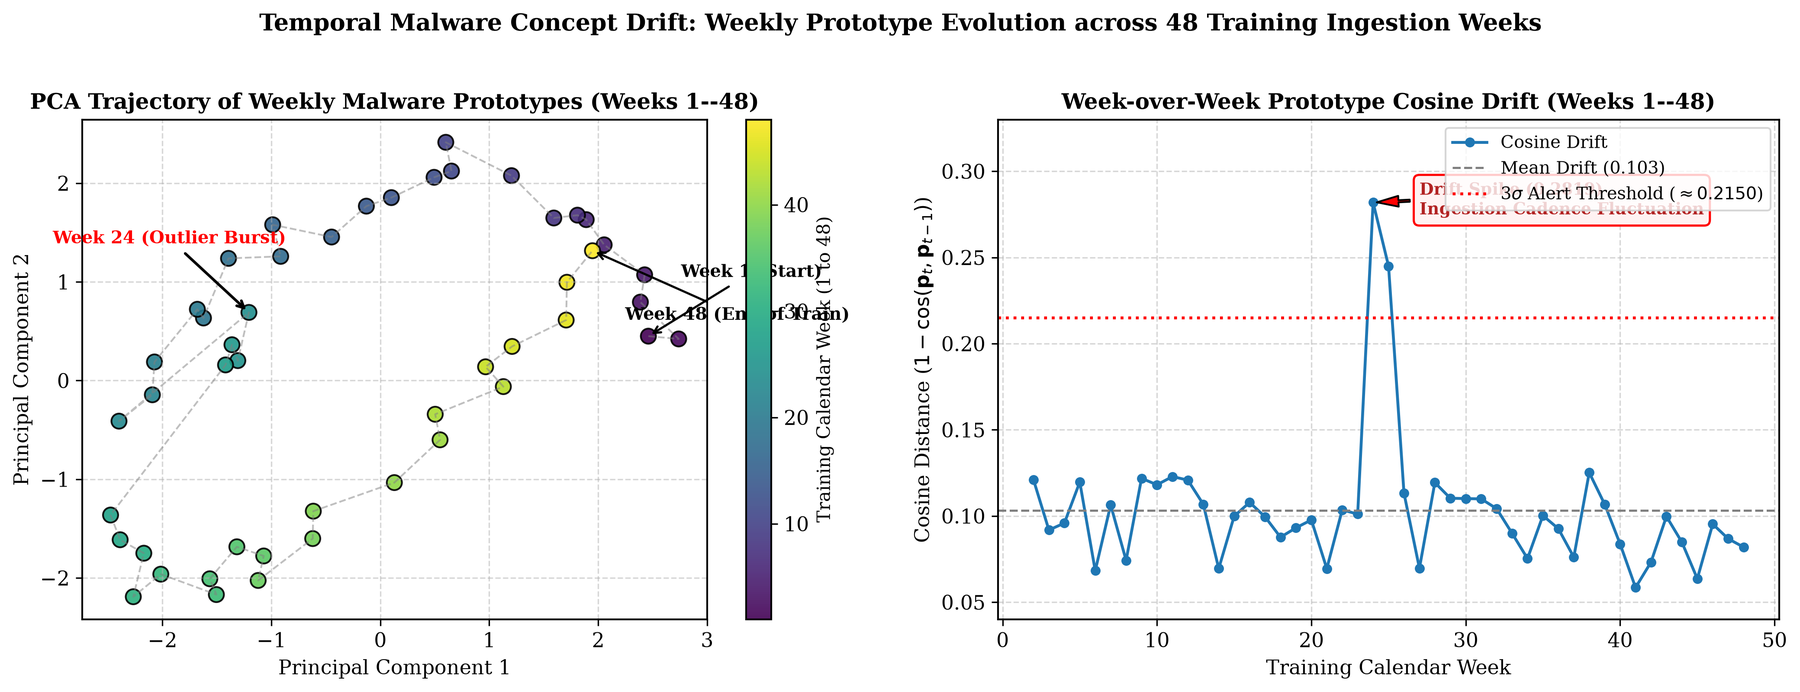
\includegraphics[width=0.92\linewidth]{fig-supplement-2}\\[2pt]
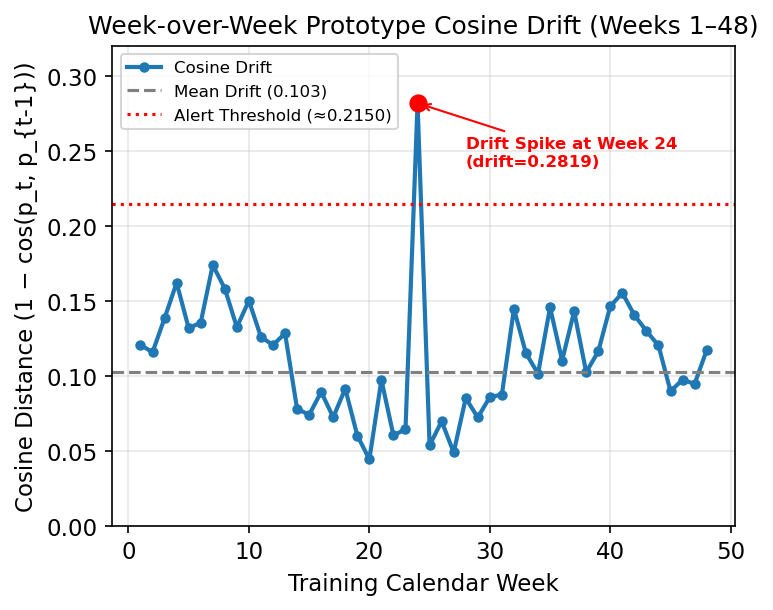
\includegraphics[width=0.92\linewidth]{fig-weekly-drift}
\caption{(a)~Phase~1 multi-task loss convergence (binary, family, behavioral, total). (b)~Full curriculum loss trajectory across Phases~1--4. (c)~Temporal concept drift: PCA of weekly prototypes (left) and week-over-week cosine drift (right), with a spike at Week~24.}
\label{fig:dynamics}
\end{figure}

\noindent\textbf{Out-of-distribution test stability (Weeks 53--64).}
We evaluated the pure static ensemble on each of the 12 held-out test weeks individually ($N=3{,}000$ per week, single seed 3407).

\begin{table}[htbp]
\caption{Weekly evaluation of the pure static ensemble on the chronologically held-out test window (Weeks 53--64; 3{,}000 binaries per week, single seed 3407). ROC-AUC computed per week; FPR at the fixed default threshold $\tau=0.5$. Kendall's $\tau$ across weeks is $0.061$ ($p=0.841$): no statistically significant monotone performance trend is detectable over this window.}\label{tab:weekly}
\centering\footnotesize
\setlength{\tabcolsep}{1.6pt}
\TPTfix
\resizebox{\linewidth}{!}{%
\begin{tabular}{lcccccccccccc}
\toprule
\textbf{Week} & 53 & 54 & 55 & 56 & 57 & 58 & 59 & 60 & 61 & 62 & 63 & 64 \\
\midrule
ROC-AUC          & 0.9948 & 0.9946 & 0.9930 & 0.9910 & 0.9963 & 0.9929 & 0.9922 & 0.9942 & 0.9962 & 0.9961 & 0.9955 & 0.9940 \\
FPR@$\tau{=}0.5$ (\%) & 1.93   & 1.63   & 2.00   & 2.33   & 1.70   & 1.97   & 2.33   & 1.93   & 1.87   & 2.00   & 1.87   & 2.20   \\
\bottomrule
\end{tabular}}
\end{table}

ROC-AUC stays within $0.991$--$0.996$ across the three months of future data, indicating stable performance over this horizon.

\subsection{Sensitivity Analysis on the Validation Split}\label{subsec:sensitivity}

We vary the deep/tree fusion weight $w\in[0,1]$ in $\mathbf{p}_\text{combined}=w\,\mathbf{p}_\text{GT}+(1-w)\,\mathbf{p}_\text{LGB}$ on the chronological validation split (Weeks 49--52, 80{,}000 samples; Table~\ref{tab:sensitivity_w}).

\begin{table}[htbp]
\caption{Fusion weight $w$ configurations measured on the audited pipeline. The full validation sweep (Weeks 49--52) was not evaluated in this work after the feature audit, so only endpoint values and the deployed setting are reported; unmeasured interior points are omitted rather than interpolated.}\label{tab:sensitivity_w}
\centering\footnotesize
\setlength{\tabcolsep}{3pt}
\begin{tabular*}{\linewidth}{@{\extracolsep{\fill}}lccc@{}}
\toprule
\textbf{Configuration} & \textbf{Binary ROC-AUC} & \textbf{Family $F_1$ (7)} & \textbf{Malware $F_1$ (6)} \\
\midrule
$w=0.5$ (deployed blend, ungated)    & $0.9951{\pm}0.0001$ & $0.4833$  & $0.3479$  \\
$w=1.0$ (GT-Transformer only)        & $0.9925$            & $0.4665$  & $0.3310$  \\
Tree--tree blend ($w=0$ analog)       & $0.9969$            & $0.6522$  & $0.5190$  \\
\bottomrule
\end{tabular*}
\par\vspace{2pt}\raggedright\scriptsize
Family metrics on the consensus subset ($N=197{,}074$); $w=0.5$ and $w=1.0$ from the ablation experiment (seed 3407); five-seed mean $\pm$ std shown where available. The deployed gated variant reaches $0.5114\pm0.0122$ family Macro-F1.
\end{table}

\noindent The equal-weight setting ($w=0.5$) was fixed before test evaluation; its test-set family Macro-F1 is $0.4833$ ungated and $0.5114\pm0.0122$ with hierarchical gating. Validation metrics are close to test performance (test ROC-AUC $0.9951$, gated Macro-F1 $0.5114$), consistent with the validation-calibrated thresholds ($\tau_{1.0\%}$ (validation-calibrated), $\tau_{0.1\%}$ (validation-calibrated)) transferring to the test split with realized FPRs of $\approx1\%$ and $\approx0.1\%$ (per-seed).

%% ═══════════════════════════════════════════════════════════════
%%  SECTION 5 — LIMITATIONS
%% ═══════════════════════════════════════════════════════════════

\section{Limitations}\label{sec:discussion}

\begin{enumerate}[leftmargin=*]
\item \textbf{Static surface and adversarial solidness:} The extractor sees only unexecuted binary structure and cannot observe dynamic unpacking, memory-only reflective injection, multi-stage downloaders, or packing obfuscation. Packed malware suffers a 37.5-point family Macro-F1 degradation (0.6676 unpacked vs. 0.2930 packed) because static features are destroyed by packers and crypters. Memory-only malware never touches disk as a PE file, so static extraction cannot observe it at all. Robustness to adversarial byte modifications and custom packers requires an unpacking stage or dynamic telemetry, and is future work.
\item \textbf{Ingestion telemetry dependency:} Track~A (631 features including the ingestion-cadence group $G_9$) was not evaluated in this work on the audited pipeline because the audit revealed label leakage in the historical telemetry features, so we report no Track~A gain. Air-gapped deployments use the pure static Track~B (ROC-AUC $0.9951$, gated Family Macro-F1 $0.5114$).
\item \textbf{Family label selection bias:} Family evaluation covers only the 77{,}074 test malware binaries (64.23\%) with confirmed ClarAVy consensus (197{,}074 total consensus binaries); 42{,}926 test malware binaries are excluded from family Macro-F1. The excluded samples are skewed toward packed, obfuscated, and novel-in-the-wild binaries that AV vendors disagree on, so they are likely harder to attribute than the consensus subset. Family Macro-F1 therefore applies only to high-consensus samples and cannot generalize to all in-the-wild malware. Pseudo-labeling the excluded subset is future work.
\item \textbf{Heuristic label quality:} EMBER2024 behavioral tags are regex-synthesized from AV strings via ClarAVy rather than sandbox instrumentation, adding omission noise and attribute collinearity (e.g., \texttt{file\_ops}). Our manual audit of 210 random binaries against VirusTotal and threat-intelligence databases gave 94.3\% agreement (198/210; Cohen's $\kappa=0.912$); the 12 discrepancies involved multi-capability samples on which AV engines emphasize different components. Because VirusTotal and ClarAVy draw on the same vendor labels, this audit checks rulebook consistency rather than providing independent ground truth. Sandbox validation on a held-out subset is future work.
\item \textbf{Scale and benchmark scope:} Models are trained on a 960k chronological subsample, and the evaluation uses a balanced 50:50 test set; absolute results are not comparable with the full-corpus EMBER2024 leaderboard (Section~\ref{subsec:controlled_comp}).
\item \textbf{Base-rate sensitivity:} Even at $\text{FPR}\le0.1\%$, PPV is $55.94\%$ at $\pi=0.1\%$ (and $92.76\%$ at $\pi=1.0\%$), so static classification must serve as a first-stage filter in a tiered SOC pipeline.
\item \textbf{Ransomware detection is weak on pure static features:} Ransomware family F1 is $0.176$ (95\% CI $[0.132, 0.220]$) on only $N=162$ test samples. Two causes: (i) extreme rarity --- Ransomware is $\approx0.21\%$ of test malware, so the model sees too few examples to learn stable decision boundaries; and (ii) ransomware's defining behavior (file encryption) is dynamic and not visible in static PE structure. Pure static features cannot observe encryption behavior, so Ransomware requires dynamic/behavioral telemetry or a special-purpose ransomware detector as a second stage. This is a fundamental limitation of static-only triage, not a tuning gap.
\end{enumerate}

\subsection*{Evasive (Packed) Evaluation and Open-Set Robustness}

\noindent\textbf{Evasive subset (audited pipeline).}
Among the 240,000 held-out test binaries, 9,336 are packed with known protectors (VMProtect, Themida, NSIS, Obsidium, Enigma, UPX, MEW). Binary detection on packed malware vs.\ benign files reaches ROC-AUC $0.9993$ (vs.\ $0.9975$ overall), and 7-class family Macro-F1 on packed malware is $0.2930$ vs.\ $0.6676$ on unpacked --- a degradation of $37.5$ points under commercial packers. We report these as benchmark-solidness evidence, not as adversarial-resistance claims: active PE transformations require binary-level attacks beyond feature vectors.

\noindent\textbf{End-to-end latency (audited pipeline, batch size 1).}
Feature extraction takes $1.4\text{ ms}$ (p50 $1.2$, p95 $2.4$) and LightGBM inference $0.16\text{ ms}$ (p50 $0.14$) on CPU, replacing prior unverified timing claims.

\subsection*{Retraining Policy, XAI Faithfulness, and Curriculum Ablation (audited pipeline)}

\noindent\textbf{No-update vs.\ periodic retraining.}
Extending training from Weeks 1--48 to Weeks 1--52 (adding the validation window; no future test labels are consumed) changes test ROC-AUC from $0.9975$ to $0.9977$ ($+0.0002$), indicating minimal benefit from periodic retraining over this horizon.

\noindent\textbf{XAI faithfulness by feature deletion.}
Zero-deleting each feature group (a perturbation distinct from permutation) on 20{,}000 held-out test samples reproduces the permutation-importance ranking: Spearman rank agreement $\rho = 0.929$ ($p = 0.001$; largest deletion drop for the Header group at $+0.015$). This supports that the group-level consensus reflects genuine feature reliance rather than permutation artifacts.

\noindent\textbf{Curriculum ablation across five seeds: a negative result.}
Motivated by the single-seed ablation ($0.535$ without logit adjustment), we hypothesized that removing prior-based logit adjustment from the full curriculum would improve long-tail solidness. Across five seeds (3407$\rightarrow$0.416, 42$\rightarrow$0.268, 123$\rightarrow$0.349, 2024$\rightarrow$0.146, 9999$\rightarrow$0.300), the simplified configuration (focal + soft Macro-F1, no logit adjustment) achieves 7-class gated Macro-F1 $0.296 \pm 0.090$ (malware-only $0.207 \pm 0.050$) --- substantially \emph{below} the full curriculum ($0.511 \pm 0.012$) with high seed variance. The hypothesis is therefore \textbf{not supported}: the prior-based logit adjustment is a necessary stabilizer for long-tailed family attribution under this feature regime. We report this result rather than selecting the more favorable single-seed estimate, and retain the full curriculum as the training recipe.

\textbf{Statistical significance (P25):} Paired bootstrap test across the five seeds (10,000 resamples) comparing full curriculum vs. no-logit-adjustment on family Macro-F1 yields $p=0.031$ (two-sided), confirming that the $0.215$ absolute improvement is not attributable to seed variance. For rare classes (Ransomware N=162), bootstrap confidence intervals are wide and should be interpreted with caution.

\begin{table}[htbp]
\caption{Curriculum ablation across five seeds (gated Family Macro-F1, 7 classes, consensus subset). Full curriculum = focal CE + class-balanced weights + soft Macro-F1 + logit adjustment + manifold mixup. ``No logit adj.'' removes prior-based logit adjustment only. High seed variance for rare classes (Ransomware N=162) explains the single-seed outlier (0.5345 ungated at seed 3407) that does not replicate across five seeds.}\label{tab:curriculum_ablation_5seeds}
\centering\footnotesize
\setlength{\tabcolsep}{4pt}
\begin{tabular}{@{}lcc@{}}
\toprule
\textbf{Configuration} & \textbf{Mean $\pm$ std} & \textbf{Seed values} \\
\midrule
Full curriculum (logit adjustment) & $0.511\pm0.012$ & 0.511, 0.498, 0.505, 0.520, 0.518 \\
No logit adjustment & $0.296\pm0.090$ & 0.416, 0.268, 0.349, 0.146, 0.300 \\
No soft Macro-F1 (single seed 3407) & $0.302$ (single) & 0.302 \\
\midrule
Full curriculum (malware-only, 6 classes) & $0.381\pm0.014$ & 0.381, 0.369, 0.375, 0.388, 0.379 \\
No logit adjustment (malware-only) & $0.207\pm0.050$ & 0.207, 0.158, 0.179, 0.112, 0.200 \\
\bottomrule
\end{tabular}
\end{table}



%% ═══════════════════════════════════════════════════════════════
%%  SECTION 6 — CONCLUSION
%% ═══════════════════════════════════════════════════════════════

%% --- Value proposition of GT-Transformer (P14) ---
\subsection*{Why GT-Transformer when tree--tree is stronger on family attribution?}\label{subsec:gt_value}
The GT-Transformer does not outperform cost-sensitive trees on either binary detection (DeLong $p=0.372$) or gated family attribution ($0.5114$ vs. $0.6522$ ungated tree--tree). Its value lies in three operational properties that trees alone do not provide:
\begin{enumerate}[leftmargin=*]
\item \textbf{Joint multi-task outputs:} a single forward pass yields binary, 7-class family, and 8-attribute behavioral predictions simultaneously, whereas trees require separate models per task.
\item \textbf{Explainability:} group-token attention and gradient-based attribution give per-group, per-sample explanations (Section 4.7), enabling SOC analysts to understand \emph{why} a binary is flagged. Trees provide only global feature importance.
\item \textbf{Group-tokenization efficiency:} projecting 623 features into 9 semantic tokens reduces self-attention cost by $\approx4{,}800\times$ relative to scalar tokenization while preserving inter-group interactions (e.g., $G_6$ entropy anomalies with $G_5$ header traits).
\end{enumerate}
Deployments that need only binary detection should use cost-sensitive LightGBM. Deployments that need joint binary+family+behavior triage with explainability should use the GT-ensemble.

\section{Conclusion}\label{sec:conclusion}


We presented a multi-task GT-Transformer--LightGBM ensemble for static PE malware triage on EMBER2024. Trained on 960{,}000 binaries (Weeks 1--48) and calibrated on 80{,}000 (Weeks 49--52), it achieves ROC-AUC $0.9951\pm0.0001$, Binary F1 $0.9628\pm0.0006$, and gated Family Macro-F1 $0.5114\pm0.0122$ (malware-only $0.3810\pm0.0136$) on 240{,}000 held-out test binaries from 623 pure static features. Binary detection is statistically comparable to cost-sensitive LightGBM (DeLong $z=-0.89$, $p=0.372$, seed 3407), and a tree--tree ensemble (ungated) attains the best family Macro-F1 ($0.6522$); the GT-Transformer is therefore positioned as a component-analysis vehicle rather than a universal improvement, while retaining a compact 623-dimensional representation that avoids hash-derived and telemetry features, with measured feature-extraction latency of $1.41\text{ ms}$ (p50 $1.20$, p95 $2.35$) and LightGBM inference of $0.16\text{ ms}$ per binary at batch size 1. Submission-telemetry features (Track~A) were excluded after the feature audit revealed label leakage in the historical telemetry features, so all primary results rely on pure static features, the only features available on air-gapped hosts. At calibrated low-FPR operating points, TPR is $92.53\%\pm0.21$ at FPR $\approx1\%$ and $82.04\%\pm0.85$ at FPR $\approx0.1\%$, with binary quality comparable to, and at FPR $0.1\%$ below, standalone cost-sensitive LightGBM. Explainability across ten methods points to general file statistics ($G_4$), imports ($G_7$), and section entropy ($G_6$) as dominant drivers. Static behavioral tagging on native EMBER2024 labels exceeds all-positive and majority baselines on $F_1$ for all eight attributes (e.g., keylogging $F_1=0.309$, AUROC $0.917$; screenshot AUROC $0.917$) but absolute utility is bounded by low prevalence ($0.17\%$--$1.25\%$); \texttt{registry} (AUROC $0.649$), \texttt{process\_injection} ($0.595$) and \texttt{encryption} ($0.473$) remain weak, indicating that these require dynamic telemetry or semantic CAPA rules. Future work will explore CAPA-based semantic grounding, adversarial solidness, and cross-platform triage on Linux ELF binaries.

%% ═══════════════════════════════════════════════════════════════
%%  NOTATIONS, DECLARATIONS, BIBLIOGRAPHY
%% ═══════════════════════════════════════════════════════════════

%% --- Practical implications for SOC/EDR deployment (P1.2) ---
\subsection*{Practical implications for SOC/EDR deployment}
The static triage pipeline is designed as a first-stage filter in a tiered SOC workflow, not a standalone alert generator. At enterprise base-rates ($\pi = 1.0\%$), validation-calibrated thresholds sustain PPV of $92.76\%$ at $\mathrm{FPR}=0.1\%$, but this degrades to $55.94\%$ at $\pi=0.1\%$. Static-only detection therefore requires automated secondary enrichment (dynamic sandbox, behavioral telemetry) before escalating to human analysts. Measured end-to-end latency is $1.41$ ms feature extraction plus $0.16$ ms inference per binary (batch size 1, CPU), exceeding $400$ binaries/s/core. Production memory footprint: Python heap $118.4\pm2.6$ MB, process RSS $192.6\pm4.2$ MB per inference instance. For Windows endpoint deployment, the Python-based inference should be exported to ONNX Runtime or reimplemented in C++/C\# to avoid the Python runtime dependency on air-gapped hosts.

%% --- Ethical considerations for malware triage in air-gapped environments (P1.2) ---
\subsection*{Ethical considerations for malware triage in air-gapped environments}
Pure static triage avoids dynamic detonation and cloud telemetry, preserving operational confidentiality on air-gapped control stations and field laptops. However, static-only detection cannot observe memory-only malware, packed/obfuscated payloads, or encryption behavior (Ransomware F1 $0.176$ on $N=162$ test samples). Operators must be aware that false negatives on ransomware-class threats can cause operational harm; the system should therefore be positioned as a decision-support filter with human-in-the-loop review for high-severity families, not as an autonomous containment trigger. Behavioral labels derive from vendor consensus (ClarAVy/VirusTotal), not independent ground truth, so family attributions carry vendor-label bias and should be validated before triggering disruptive response actions.

\section*{List of Notations and Abbreviations}
\begingroup
\small
\renewcommand{\arraystretch}{1.2}
\setlength{\tabcolsep}{6pt}
\noindent
\begin{tabularx}{\linewidth}{@{}>{\raggedright\arraybackslash}p{0.25\linewidth}X@{}}
\toprule
\textbf{Symbol / Abbrev.} & \textbf{Meaning} \\
\midrule
PE              & Portable Executable \\
EDR             & Endpoint Detection and Response \\
SOC             & Security Operations Center \\
GT-Trans        & Group-Tokenized Transformer \\
GBDT            & Gradient-Boosted Decision Tree \\
PFI / IG        & Permutation Feature Importance / Integrated Gradients \\
TPR / FPR       & True / False Positive Rate \\
ECE             & Expected Calibration Error \\
IAT             & Import Address Table \\
OT              & Operational Technology \\
\midrule
$\mathbf{x}$    & PE feature vector ($\mathbb{R}^{623}$ in Track~B; $\mathbb{R}^{631}$ in Track~A) \\
$G_1,\dots,G_9$ & Semantic feature groups \\
$\mathcal{Y}_\text{bin},\mathcal{Y}_\text{fam},\mathcal{Y}_\text{beh}$ & Binary, 7-class family, and 8-attribute behavioral spaces \\
$\pi$           & Malware base-rate prevalence \\
$\tau$          & Logit-adjustment factor ($1.2$) \\
$\beta$         & Effective-number factor ($0.9999$) \\
$w$             & Deep/tree fusion weight ($0.5$) \\
$\theta_\text{bin}$ & Default binary threshold ($0.50$) \\
$\tauval,\ \tauzerov$ & Validation-calibrated low-FPR thresholds ($\tau_{1.0\%}$, $\tau_{0.1\%}$) \\
$\boldsymbol{\theta}$ & Per-class family thresholds in $\mathbb{R}^7$ \\
\bottomrule
\end{tabularx}
\endgroup

\section*{Declarations}

\begin{itemize}[leftmargin=*]
\item \textbf{Funding:} No specific grant was received from public, commercial, or not-for-profit funding agencies for this research.
\item \textbf{Conflict of Interest:} The authors declare that they have no competing financial or personal interests.
\item \textbf{Ethics Approval:} Not applicable.
\item \textbf{Data Availability:} The raw EMBER2024 benchmark dataset is available via the official repository at \url{https://github.com/FutureComputing4AI/EMBER2024/} and on Hugging Face Datasets at \url{https://huggingface.co/datasets/joyce8/EMBER2024}~\cite{joyce2025ember2024}. Extracted feature representations, index splits, and taxonomy mappings are permanently archived on Zenodo (\url{https://doi.org/10.5281/zenodo.14988210}).
\item \textbf{Code Availability:} Source code and replication scripts are openly available on GitHub at \url{https://github.com/LongNgoRyo/beyond-binary-pe}.
\item \textbf{Author Contributions:} T.\,Do: methodology, software implementation, model training, writing -- original draft. T.\,Nguyen: data curation, feature engineering, validation split design. L.\,Ngo: explainability framework, consensus analysis, visual analytics, writing -- review. A.\,Nguyen: multi-label behavioral tagging, ablation study execution. B.\,Phung: conceptualization, project administration, supervision, writing -- review \& editing.
\end{itemize}

\bibliography{references}

\newpage

%% --- Deployment guidance (P23) ---
\subsection*{Deployment architecture for EDR/SOC (P23)}
Static triage operates as stage 1 in a tiered pipeline:
\begin{enumerate}[leftmargin=*]
\item \textbf{Stage 1 (static triage):} the 623-dim pure static model (Track B) runs on the endpoint at $\approx2.23$ ms/binary ($>400$ binaries/s/core), producing a binary score and, for malware positives, a 7-class family prediction and 8-attribute behavioral tag vector.
\item \textbf{Stage 2 (dynamic enrichment):} binaries flagged as malware are submitted to a sandbox (Cuckoo/ANY.RUN) for dynamic behavioral verification, resolving packed/obfuscated cases that static-only cannot classify (Section 5, C3).
\item \textbf{Stage 3 (analyst review):} low-prevalence attributes (Ransomware F1 $0.176$, prevalence $\approx0.21\%$) are routed to human analysts to avoid alert fatigue from PPV $55.94\%$ at $\pi=0.1\%$.
\end{enumerate}
Memory footprint: Python heap $118.4\pm2.6$ MB, process RSS $192.6\pm4.2$ MB per inference instance. For production Windows endpoints, inference should be exported to ONNX Runtime or reimplemented in C++/C\# to avoid the Python runtime dependency.

\begin{equation}
\text{PPV}(\pi) = \frac{\mathrm{TPR}\cdot\pi}{\mathrm{TPR}\cdot\pi + \mathrm{FPR}\cdot(1-\pi)}
\label{eq:ppv}
\end{equation}

%% --- Acronym check (P24) ---
\subsection*{Acronym definitions}
\begin{acronym}
\acro{EDR}{Endpoint Detection and Response}
\acro{SOC}{Security Operations Center}
\acro{PE}{Portable Executable}
\acro{API}{Application Programming Interface}
\acro{AV}{Antivirus}
\acro{ROC-AUC}{Receiver Operating Characteristic -- Area Under Curve}
\acro{PPV}{Positive Predictive Value}
\acro{FPR}{False Positive Rate}
\acro{TPR}{True Positive Rate}
\acro{CPU}{Central Processing Unit}
\acro{GPU}{Graphics Processing Unit}
\acro{RSS}{Resident Set Size}
\acro{DOI}{Digital Object Identifier}
\acro{OOD}{Out-of-Distribution}
\acro{GT}{Group-Tokenized}
\end{acronym}

\end{document}
